\mychapter{집합}{}
\section{집합과 원소}
\subsection{집합과 원소의 정의와 포함 관계}
어떤 기준에 의하여 그 대상을 분명히 알 수 있는 것들의 모임을 \term{집합}{}이라고 합니다. 이때 집합을 이루는 대상 하나하나를 그 집합의 \term{원소}{}라고 합니다. 일반적으로 집합은 대문자 $A$, $B$, $C$로 나타내고, 원소는 소문자 $a$, $b$, $c$로 나타냅니다.

$a$가 집합 $A$의 원소일 때, `$a$는 집합 $A$에 \term{속한다}{}'고 하며, 이것을 기호로 $a \in A$와 같이 나타냅니다. $b$가 집합 $A$의 원소가 아닐 때, `$b$는 집합 $A$에 \term{속하지 않는다}{}'고 하며, 이것을 기호로 $b \not\in A$와 같이 나타냅니다. 

\subsection{집합의 서로 같음}
두 집합 $A$, $B$에 대하여 $A$의 모든 원소가 $B$에 속하고,  $B$의 모든 원소가 $A$에 속할 때, $A$, $B$는 \term{서로 같다}{}고 하며, $A=B$라 표기합니다. 두 집합 $A$, $B$가 서로 같지 않을 때는 $A \neq B$라 표기합니다.

\subsection{공집합}
원소를 하나도 갖지 않는 집합을 \term{공집합}{}이라고 하며, $\emptyset$라 표기합니다. 

\subsection{원소의 개수}
원소의 개수가 유한개인 집합 $A$에 대하여 $A$에 속하는 원소의 개수를 $n\left( A \right) $라 표기합니다. 공집합의 원소의 개수는 정의에 의하여 $0$이므로 $n\left( \emptyset \right)=0$입니다. 한편, 원소의 개수가 무수히 많은 집합에 대해서는 원소의 개수를 따지지 않습니다.

\subsection{집합의 표현}
집합에 포함된 원소가 무엇인지 표현하는 방법은 세 가지가 있습니다. $n\left( A \right) = 4$이고 $1 \in A$, $2 \in A$, $4 \in A$, $8 \in A$인 집합 $A$를 세 가지 방법으로 나타내봅시다.

첫 번째 방법은 집합에 속하는 모든 원소를 나열하는 방법(\term{원소나열법}{})입니다. 집합에 속하는 모든 원소를 중괄호 기호 \{ \} 사이에 하나하나 나열하여 적되, 중복된 원소가 없도록 하고, 나열된 원소에 일정한 규칙이 있다면 중간을 $\cdots$로 생략할 수 있습니다. 이 방법에 따르면 $A=\left\{ 1,\:2,\:4,\:8 \right\} $입니다. 

두 번째 방법은 집합에 속하는 모든 원소들이 갖는 공통적 성질을 조건\mn{조건이라는 용어는 \mbox{Zero 1.4)}에서 배웁니다.}으로 제시하는 방법(\term{조건제시법}{})입니다.  이 방법에 따르면 $1$, $2$, $4$, $8$은 모두 $8$의 약수라는 공통적 성질을 갖고 있으므로 $A=\conset{x}{$x$는 $8$의 약수}$입니다. 
\cleartorecto\begin{center}
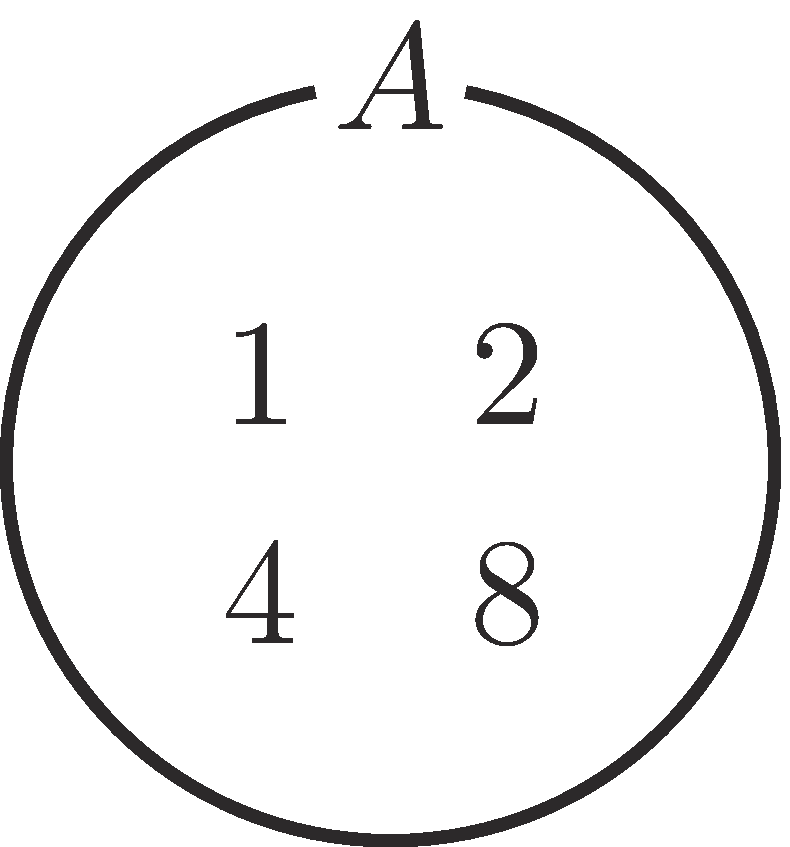
\includegraphics[scale=\pgfkeysvalueof{picsize}]{DBs/pic/zero_01.pdf}\
\end{center}세 번째 방법은 그림을 이용한 방법(\term{벤 다이어그램}{})입니다. 그림과 같이 집합을 원으로 표시하고, 원소를 원 안에 나열하는 것입니다.
\section{집합 사이의 포함 관계}

\subsection{부분집합과 진부분집합}
두 집합 $A$, $B$에 대하여 $A$의 모든 원소가 $B$에 속할 때, $A$를 $B$의 \term{부분집합}{}이라고 하며, $A \subset B$라 표기합니다. 한편 $A$의 원소 중에서 단 하나라도 $B$에 속하지 않는 원소가 있으면 $A$는 $B$의 부분집합이 아니며, 이를 $A \not\subset B$라 표기합니다.

집합 $A$의 모든 원소는 자기 자신인 $A$에 속하므로, 모든 집합은 자기 자신의 부분집합입니다. 또한 공집합은 모든 집합의 부분집합입니다.

어떤 집합에 대하여, 자기 자신이 아닌 부분집합을 그 집합의 \term{진부분집합}{}이라고 합니다. 즉 두 집합 $A$, $B$에 대하여 $A \subset B$이고 $A \neq B$일 때, $A$는 $B$의 진부분집합입니다.

\begin{remark}{부분집합의 개수와 진부분집합의 개수}
사실 이 내용은 확률과 통계의 `경우의 수'에서 다루지만, 어렵지 않은 내용이므로 가볍게 다루어봅시다.

$n\left( A \right) = k $인 집합의 원소를 각각 $a_1$, $a_2$, $\cdots$, $a_k$라 할 때, $A$의 부분집합 $B$에는 $a_1$이 속할 수도 있고, 속하지 않을 수도 있습니다. 이는 $a_2$, $a_3$, $\cdots$, $a_k$ 모두 마찬가지이고, 각각의 사건은 서로 동시에(잇달아) 일어납니다. 따라서 곱의 법칙에 의하여 $k$개의 $2$를 서로 곱하면 $2\times2\times\cdots\times2=2^k$이므로 서로 다른 $B$의 개수는 $2^k$입니다. 진부분집합의 개수는 이 값에서 `집합 자기 자신의 개수'인 $1$을 뺀 $2^k -1$입니다.
\end{remark}
\vskip-20pt
\subsection{두 집합 사이의 포함 관계}
\vskip-10pt
\begin{figure}[h]\centering \subfloat[][]{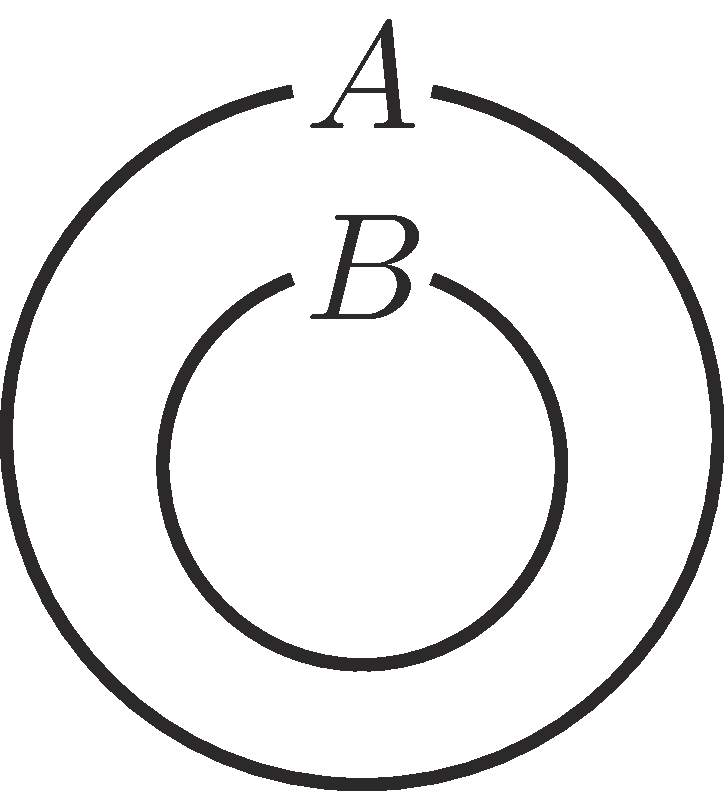
\includegraphics[scale=\pgfkeysvalueof{picsize}]{DBs/pic/zero_02_1.pdf}}\
\qquad
\centering \subfloat[][]{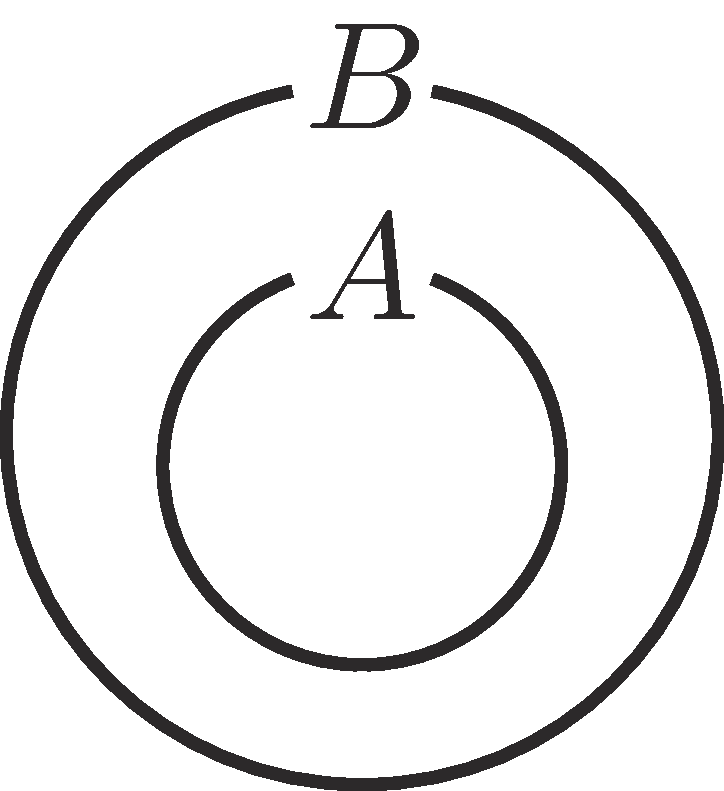
\includegraphics[scale=\pgfkeysvalueof{picsize}]{DBs/pic/zero_02_2.pdf}}\
\qquad
\centering \subfloat[][]{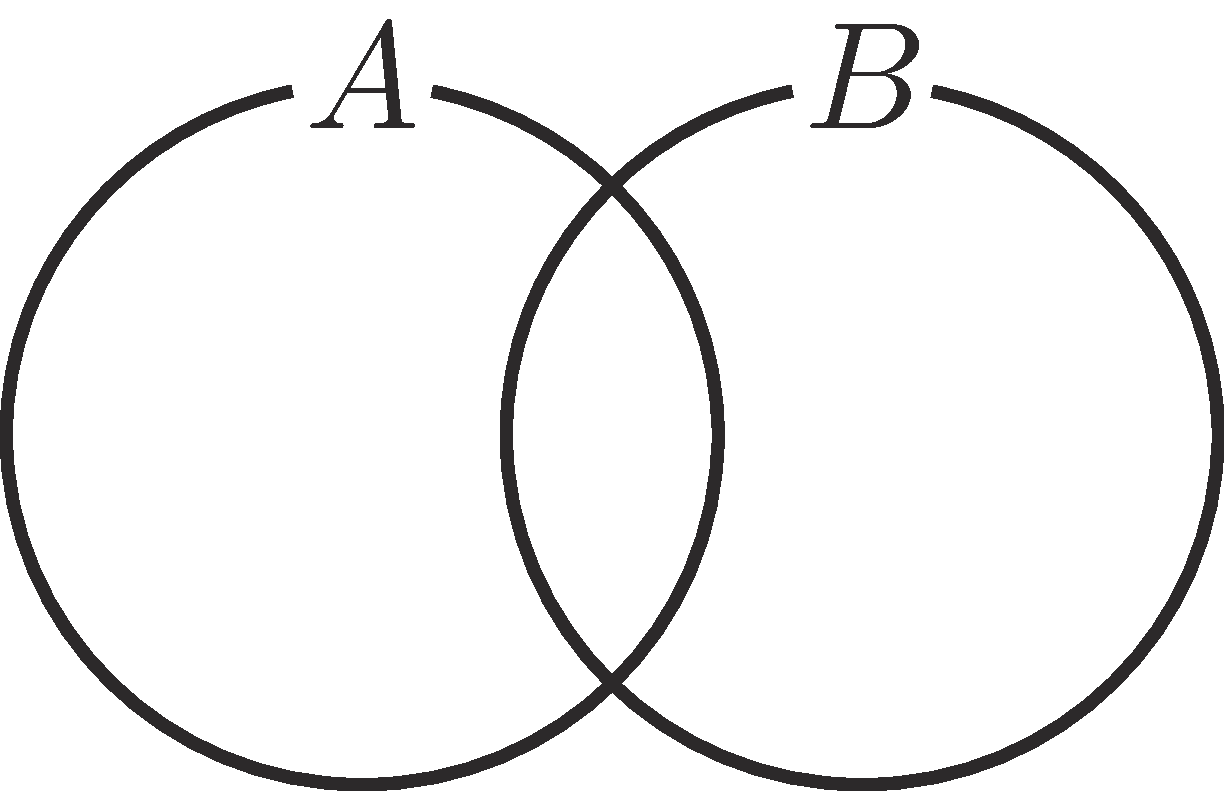
\includegraphics[scale=\pgfkeysvalueof{picsize}]{DBs/pic/zero_02_3.pdf}}\\
\centering \subfloat[][]{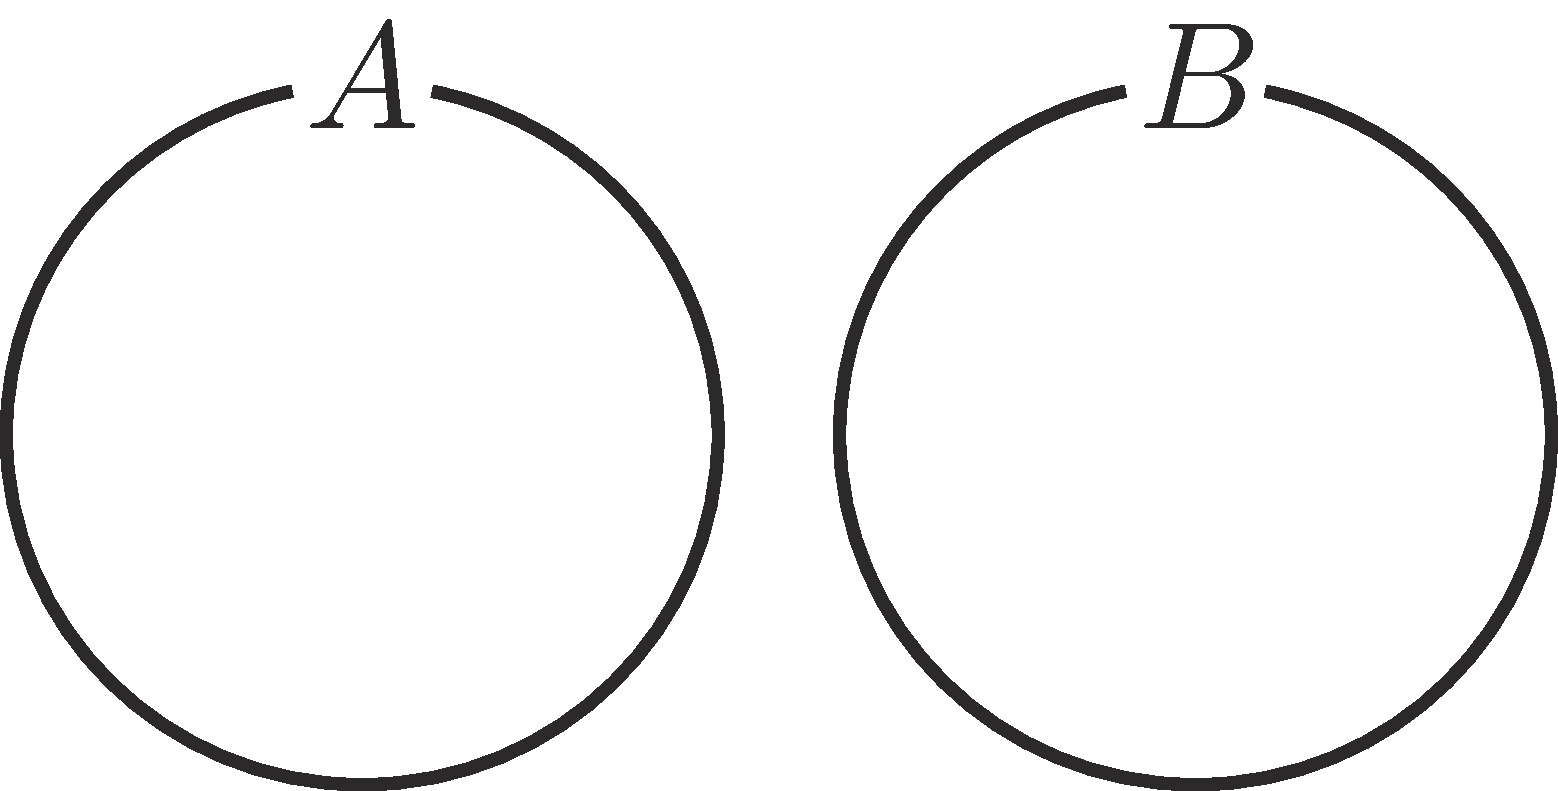
\includegraphics[scale=\pgfkeysvalueof{picsize}]{DBs/pic/zero_02_4.pdf}}\
\qquad
\centering \subfloat[][]{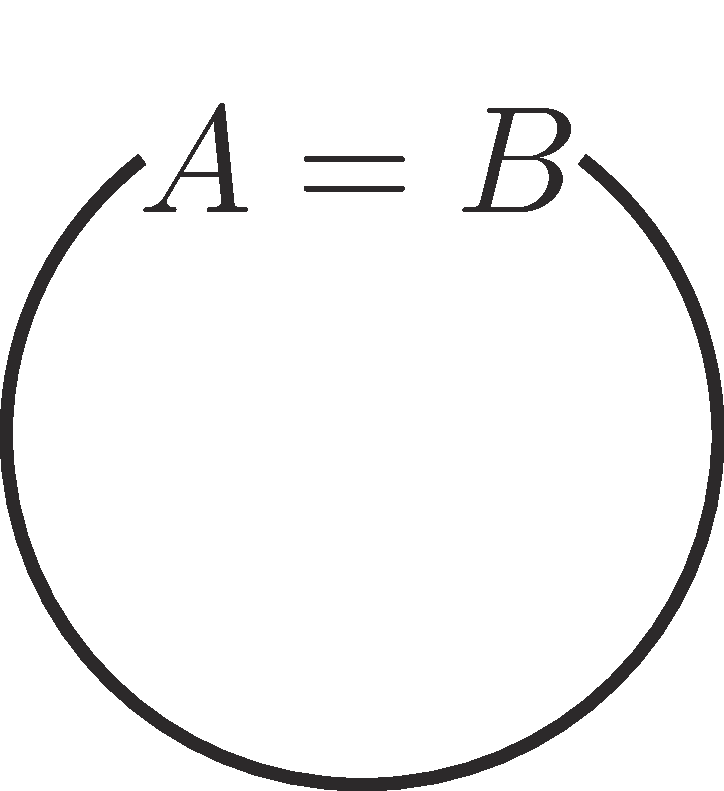
\includegraphics[scale=\pgfkeysvalueof{picsize}]{DBs/pic/zero_02_5.pdf}}\
\end{figure}\vskip-10pt


두 집합 $A$, $B$ 사이의 포함 관계는 그림과 같이 다섯 가지가 있습니다. (a), (b)는 한 집합이 다른 집합의 진부분집합인 경우입니다. (c)는 각 집합이 일부 원소만을 공유하는 경우입니다. (d)는 각 집합이 공유하는 원소가 없는 경우입니다. (e)는 두 집합이 서로 같은 경우입니다.

\section{집합의 연산}
\subsection{교집합, 합집합, 서로소}
\begin{center} 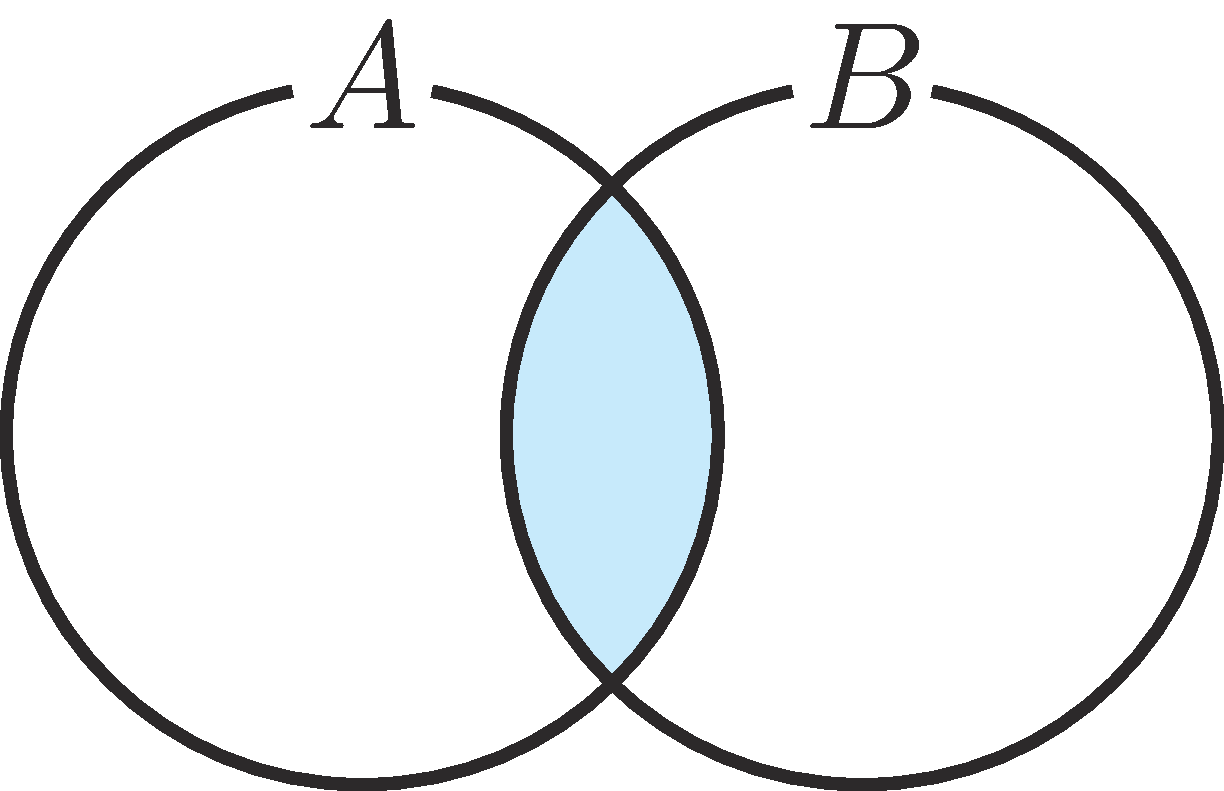
\includegraphics[scale=\pgfkeysvalueof{picsize}]{DBs/pic/zero_03.pdf}\
	\end{center}두 집합 $A$, $B$의 포함관계가 그림과 같을 때, 색칠된 부분은 $A$에도 속하고 $B$에도 속하는 원소들을 나타냅니다. 이러한 모든 원소로 이루어진 집합을 `$A$와 $B$의 \term{교집합}{}'이라 하며, $A \cap B$라 표기합니다. 이를 조건제시법으로 나타내면 다음과 같습니다.\mn{`속하고'라는 표현이 `그리고'로 바뀌는 것에 주목할 필요가 있습니다.}{} \begin{align*}A\cap B = \conset{x}{$x\in A$ 그리고 $x\in B$} \end{align*}
\begin{center} 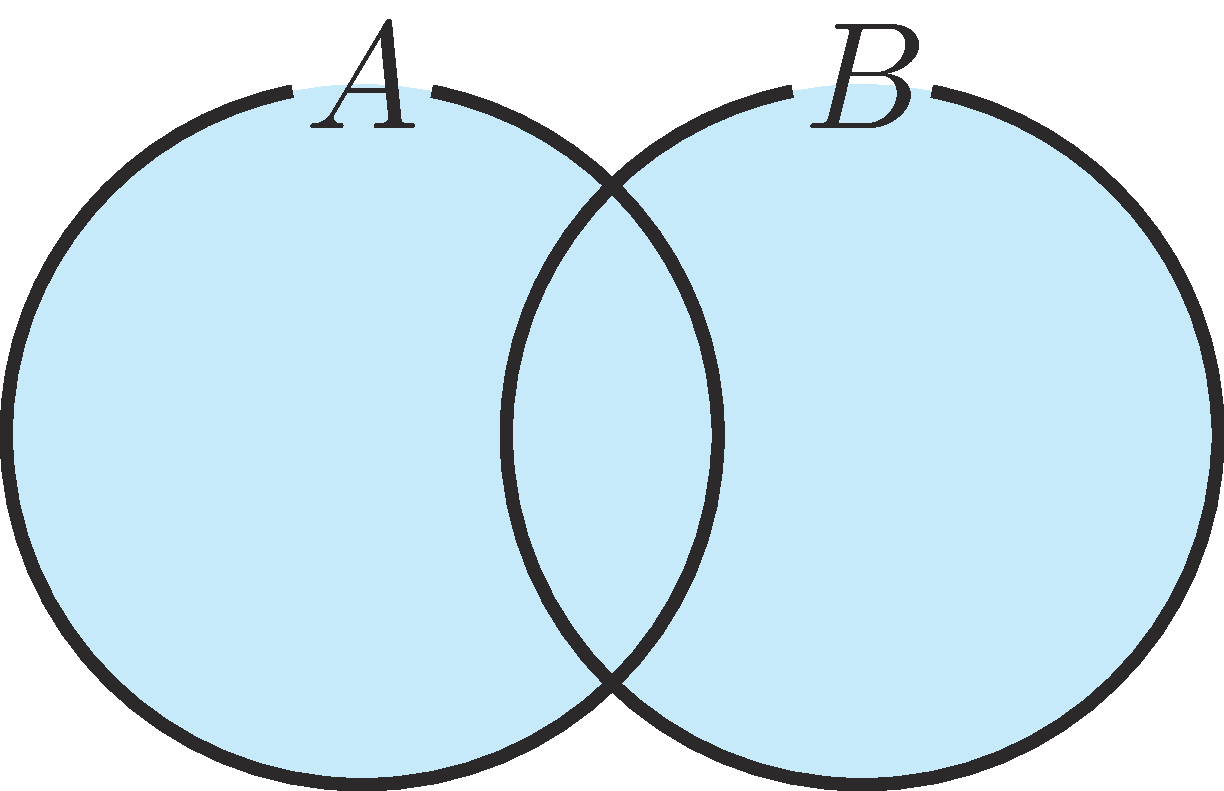
\includegraphics[scale=\pgfkeysvalueof{picsize}]{DBs/pic/zero_04.pdf}\
	\end{center}두 집합 $A$, $B$의 포함관계가 그림과 같을 때, 색칠된 부분은 $A$에 속하거나 $B$에 속하는 원소들을 나타냅니다. 이러한 모든 원소로 이루어진 집합을 `$A$와 $B$의 \term{합집합}{}'이라 하며, $A \cup B$라 표기합니다. 이를 조건제시법으로 나타내면 다음과 같습니다.\mn{`속하거나'라는 표현이 `또는'으로 바뀌는 것에 주목할 필요가 있습니다.}{} \begin{align*}A\cup B = \conset{x}{$x\in A$ 또는 $x\in B$} \end{align*}
\begin{center} 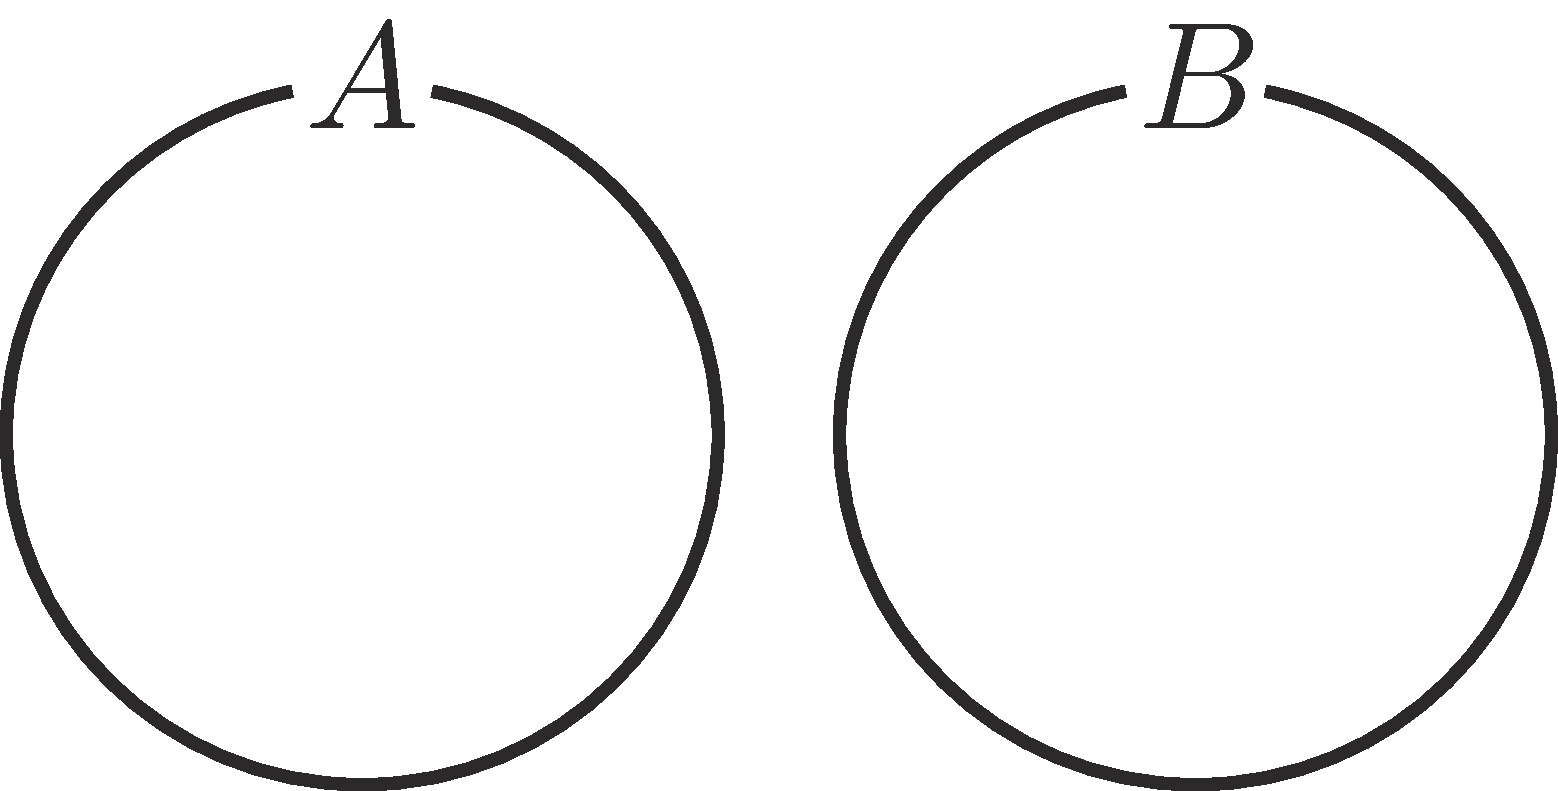
\includegraphics[scale=\pgfkeysvalueof{picsize}]{DBs/pic/zero_05.pdf}\
	\end{center}두 집합 $A$, $B$의 포함관계가 그림과 같아서 각 집합이 공유하는 원소가 없을 때, 즉 $A \cap B = \emptyset$인 경우, 두 집합 `$A$와 $B$는 \term{서로소}{}'라고 합니다.

\subsection{합집합의 원소의 개수}
원소의 개수가 유한개인 두 집합 $A$, $B$에 대하여 다음이 성립합니다.
\begin{align*}n\left( A\cup B \right) = n\left( A \right)  + n\left( B \right) - n\left( A \cap B \right)\end{align*}
\clearpage
\subsection{차집합}
\begin{center} 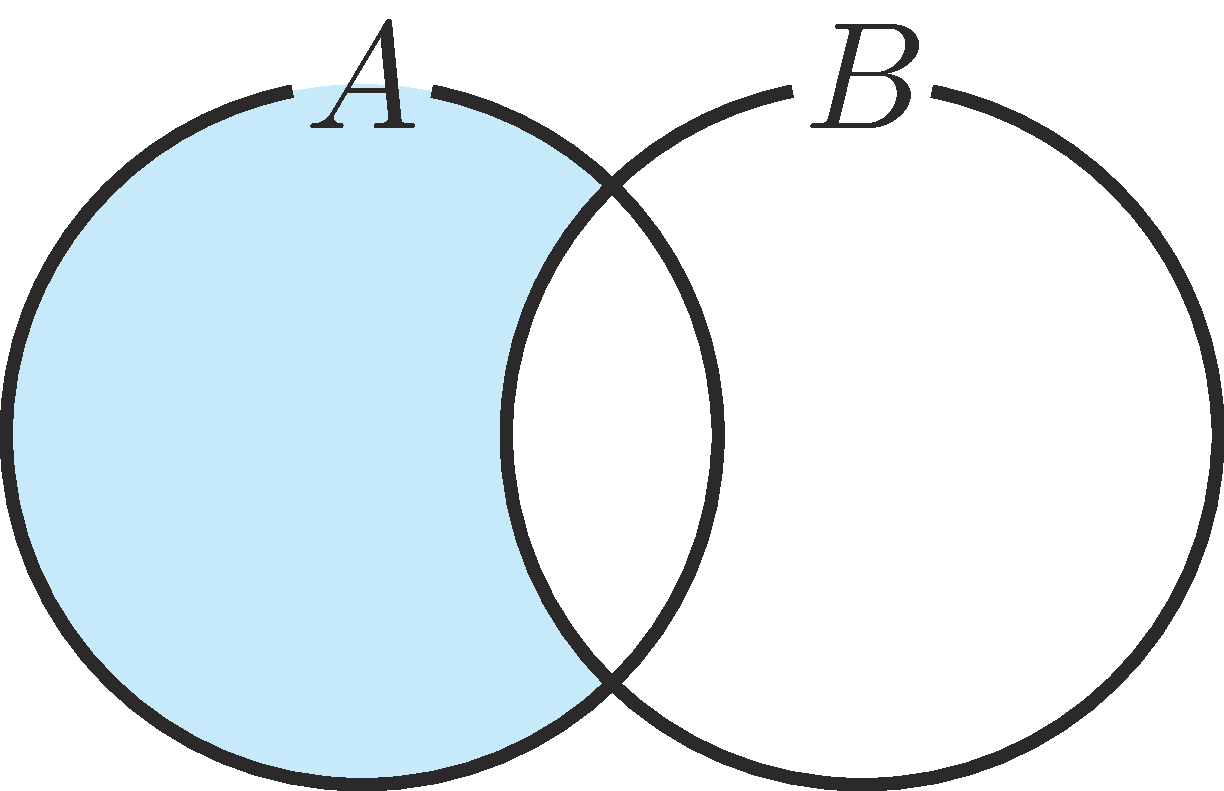
\includegraphics[scale=\pgfkeysvalueof{picsize}]{DBs/pic/zero_06.pdf}\
	\end{center}두 집합 $A$, $B$의 포함관계가 그림과 같을 때, 색칠된 부분은 $A$에는 속하고 $B$에는 속하지 않는 원소들을 나타냅니다. 이러한 모든 원소로 이루어진 집합을 `$A$에 대한 $B$의 \term{차집합}{}'이라 하며, $A - B$라 표기합니다. 이를 조건제시법으로 나타내면 다음과 같습니다.\mn{`속하고'라는 표현이 `그리고'로 바뀌는 것에 주목할 필요가 있습니다.}{} \begin{align*}A - B = \conset{x}{$x\in A$ 그리고 $x\not\in B$} \end{align*}

\subsection{전체집합과 여집합}
\begin{center} 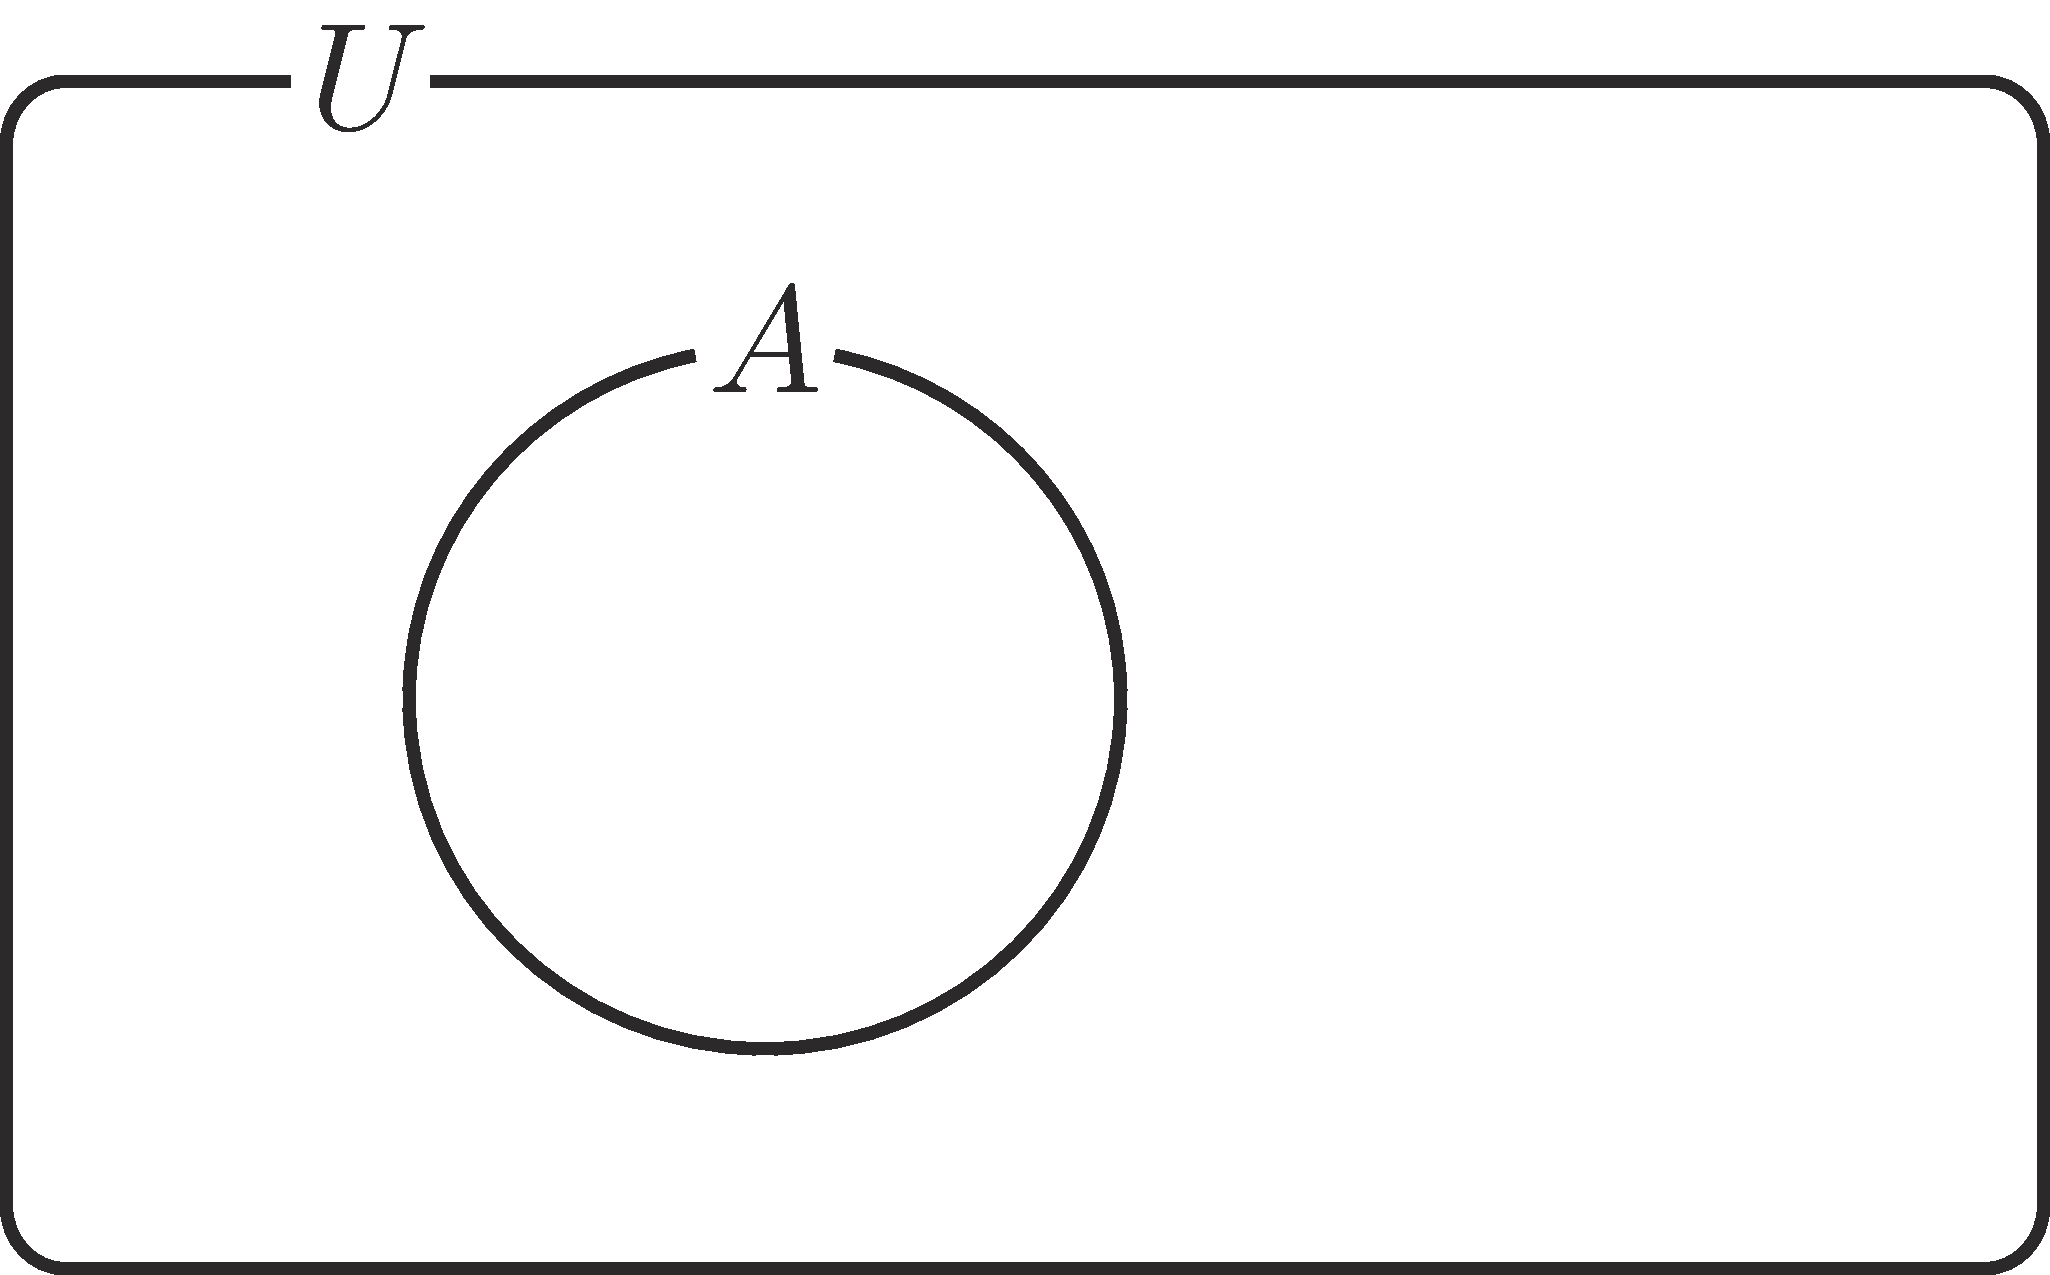
\includegraphics[scale=\pgfkeysvalueof{picsize}]{DBs/pic/zero_07.pdf}\
	\end{center}주어진 어떤 집합에 대하여 그의 부분집합을 생각할 때, 처음에 주어진 집합을 \term{전체집합}{}이라고 하며, $U$라 표기합니다. 전체집합을 벤 다이어그램에 나타낼 때, 관습적으로 모서리가 둥근 네모꼴로 나타냅니다.
\begin{center} 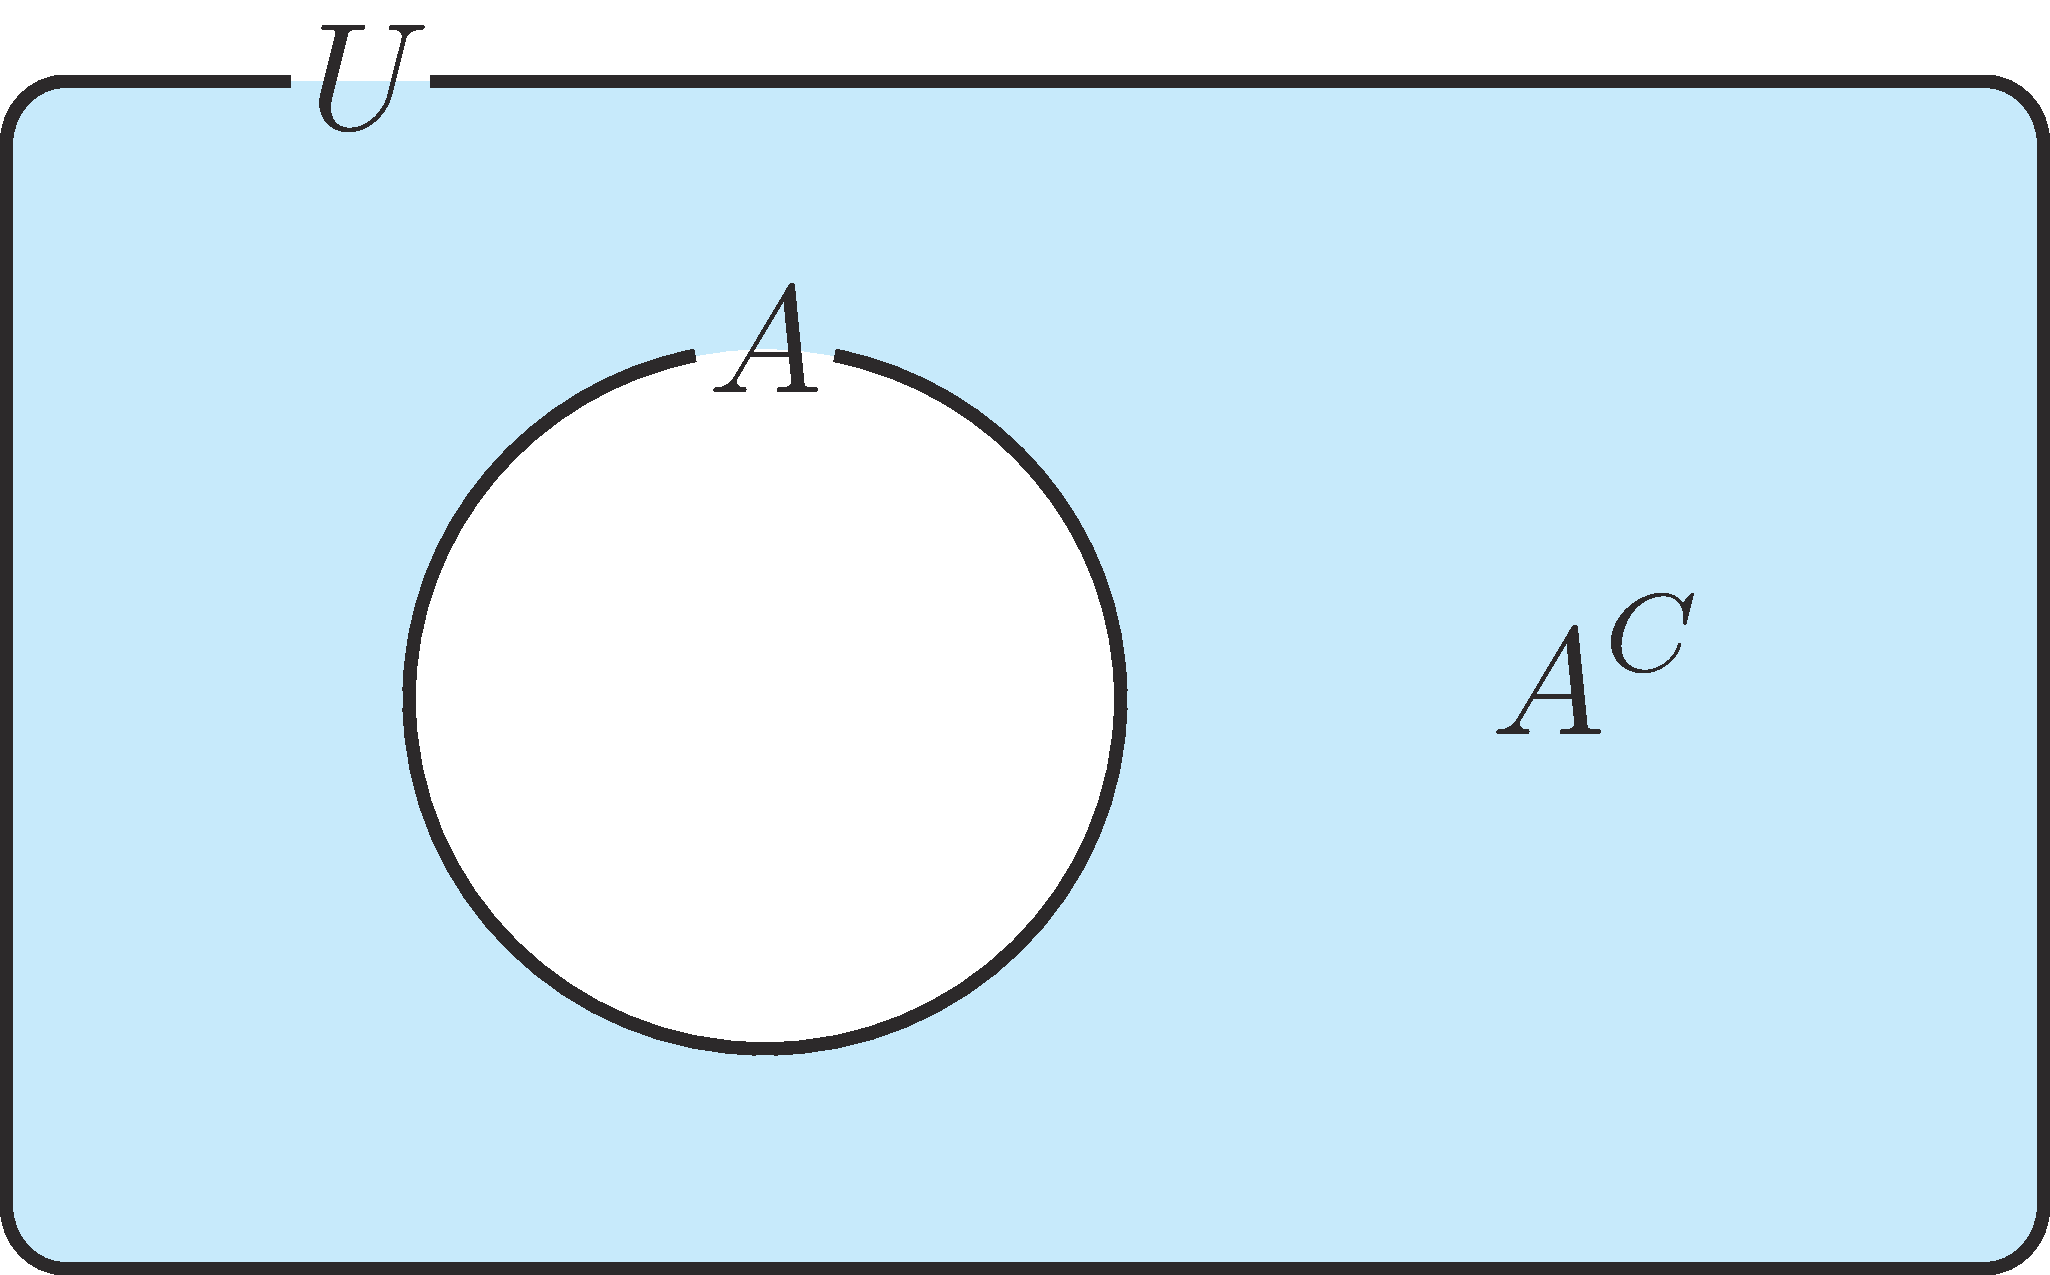
\includegraphics[scale=\pgfkeysvalueof{picsize}]{DBs/pic/zero_08.pdf}\
	\end{center}전체집합 $U$의 부분집합 $A$에 대하여 $U$의 원소 중에서 $A$에 속하지 않는 모든 원소로 이루어진 집합을 `$U$에 대한 $A$의 \term{여집합}{}'이라고 하며, $A^C$라 표기합니다. 이를 조건제시법으로 나타내면 다음과 같습니다.\begin{align*}A^C= \conset{x}{$x\in U$ 그리고 $x\not\in A$} \end{align*}

\clearpage
\section{집합의 연산}
\subsection{전체집합, 여집합, 차집합의 연산}
\begin{center} 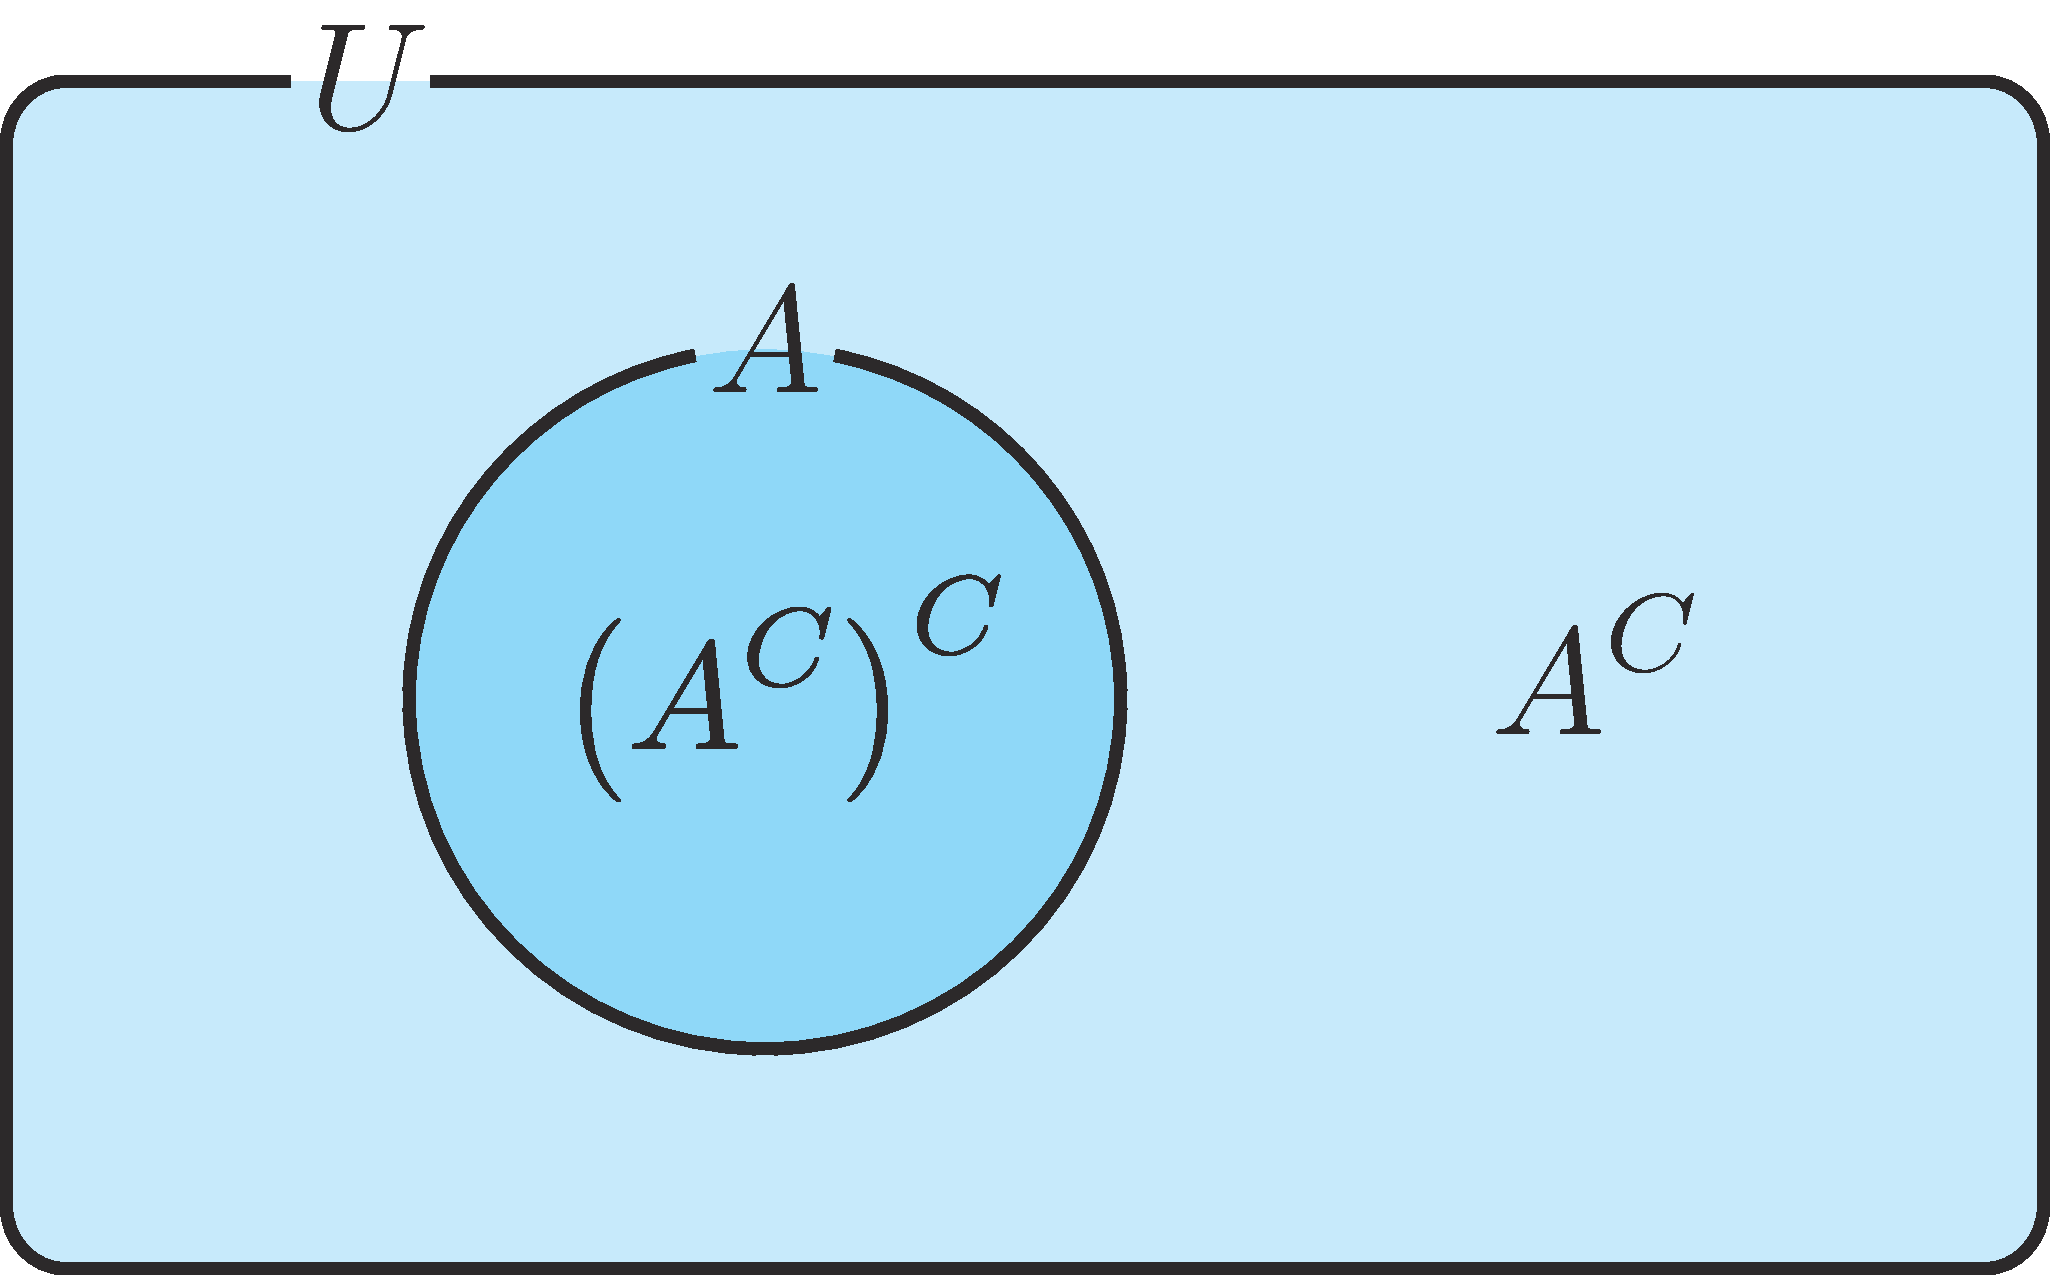
\includegraphics[scale=\pgfkeysvalueof{picsize}]{DBs/pic/zero_09.pdf}\
	\end{center}전체집합 $U$의 부분집합 $A$에 대하여, $A\cup A^C = U$, $\left( A^C \right)^C = A $가 성립합니다. 위 그림은 이 연산을 벤 다이어그램으로 나타낸 것입니다.
\begin{center} 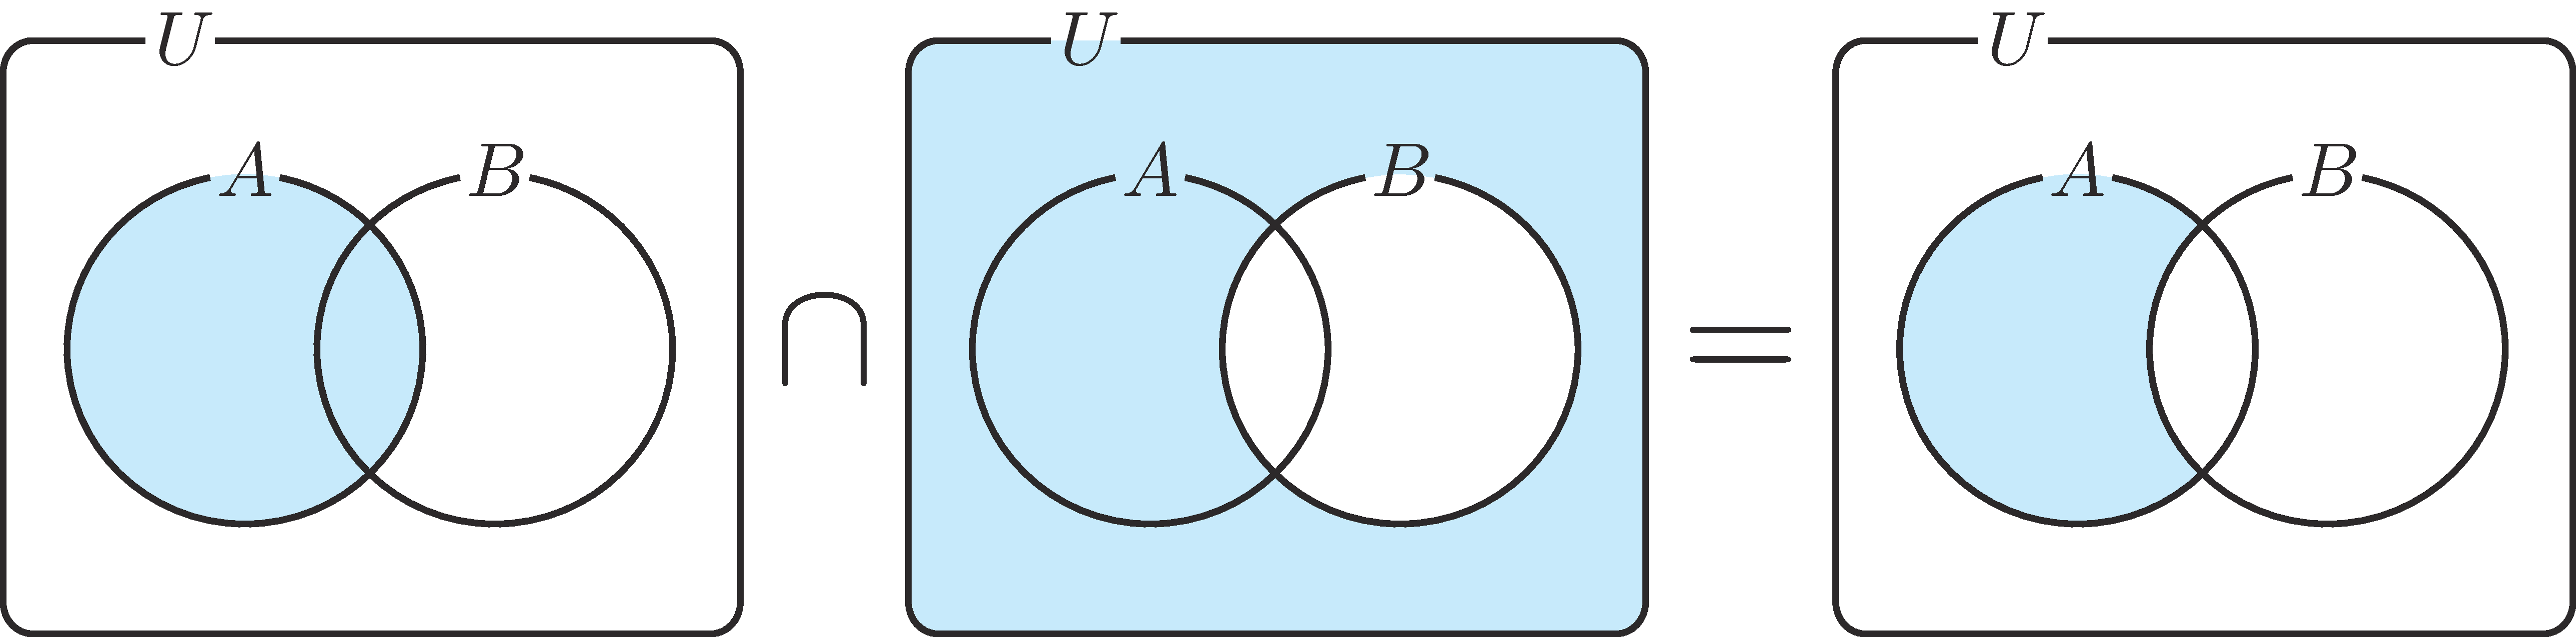
\includegraphics[scale=\pgfkeysvalueof{picsize}]{DBs/pic/zero_10.pdf}\
	\end{center}전체집합 $U$에 속하는 두 집합 $A$, $B$의 포함관계가 그림과 같은 경우, 여집합 기호와 집합의 연산을 이용하여 $A$에 대한 $B$의 차집합을 $A\cap B^C$와 같이 표현할 수 있습니다. 위 그림은 이 연산을 벤 다이어그램으로 나타낸 것입니다.
\begin{center} 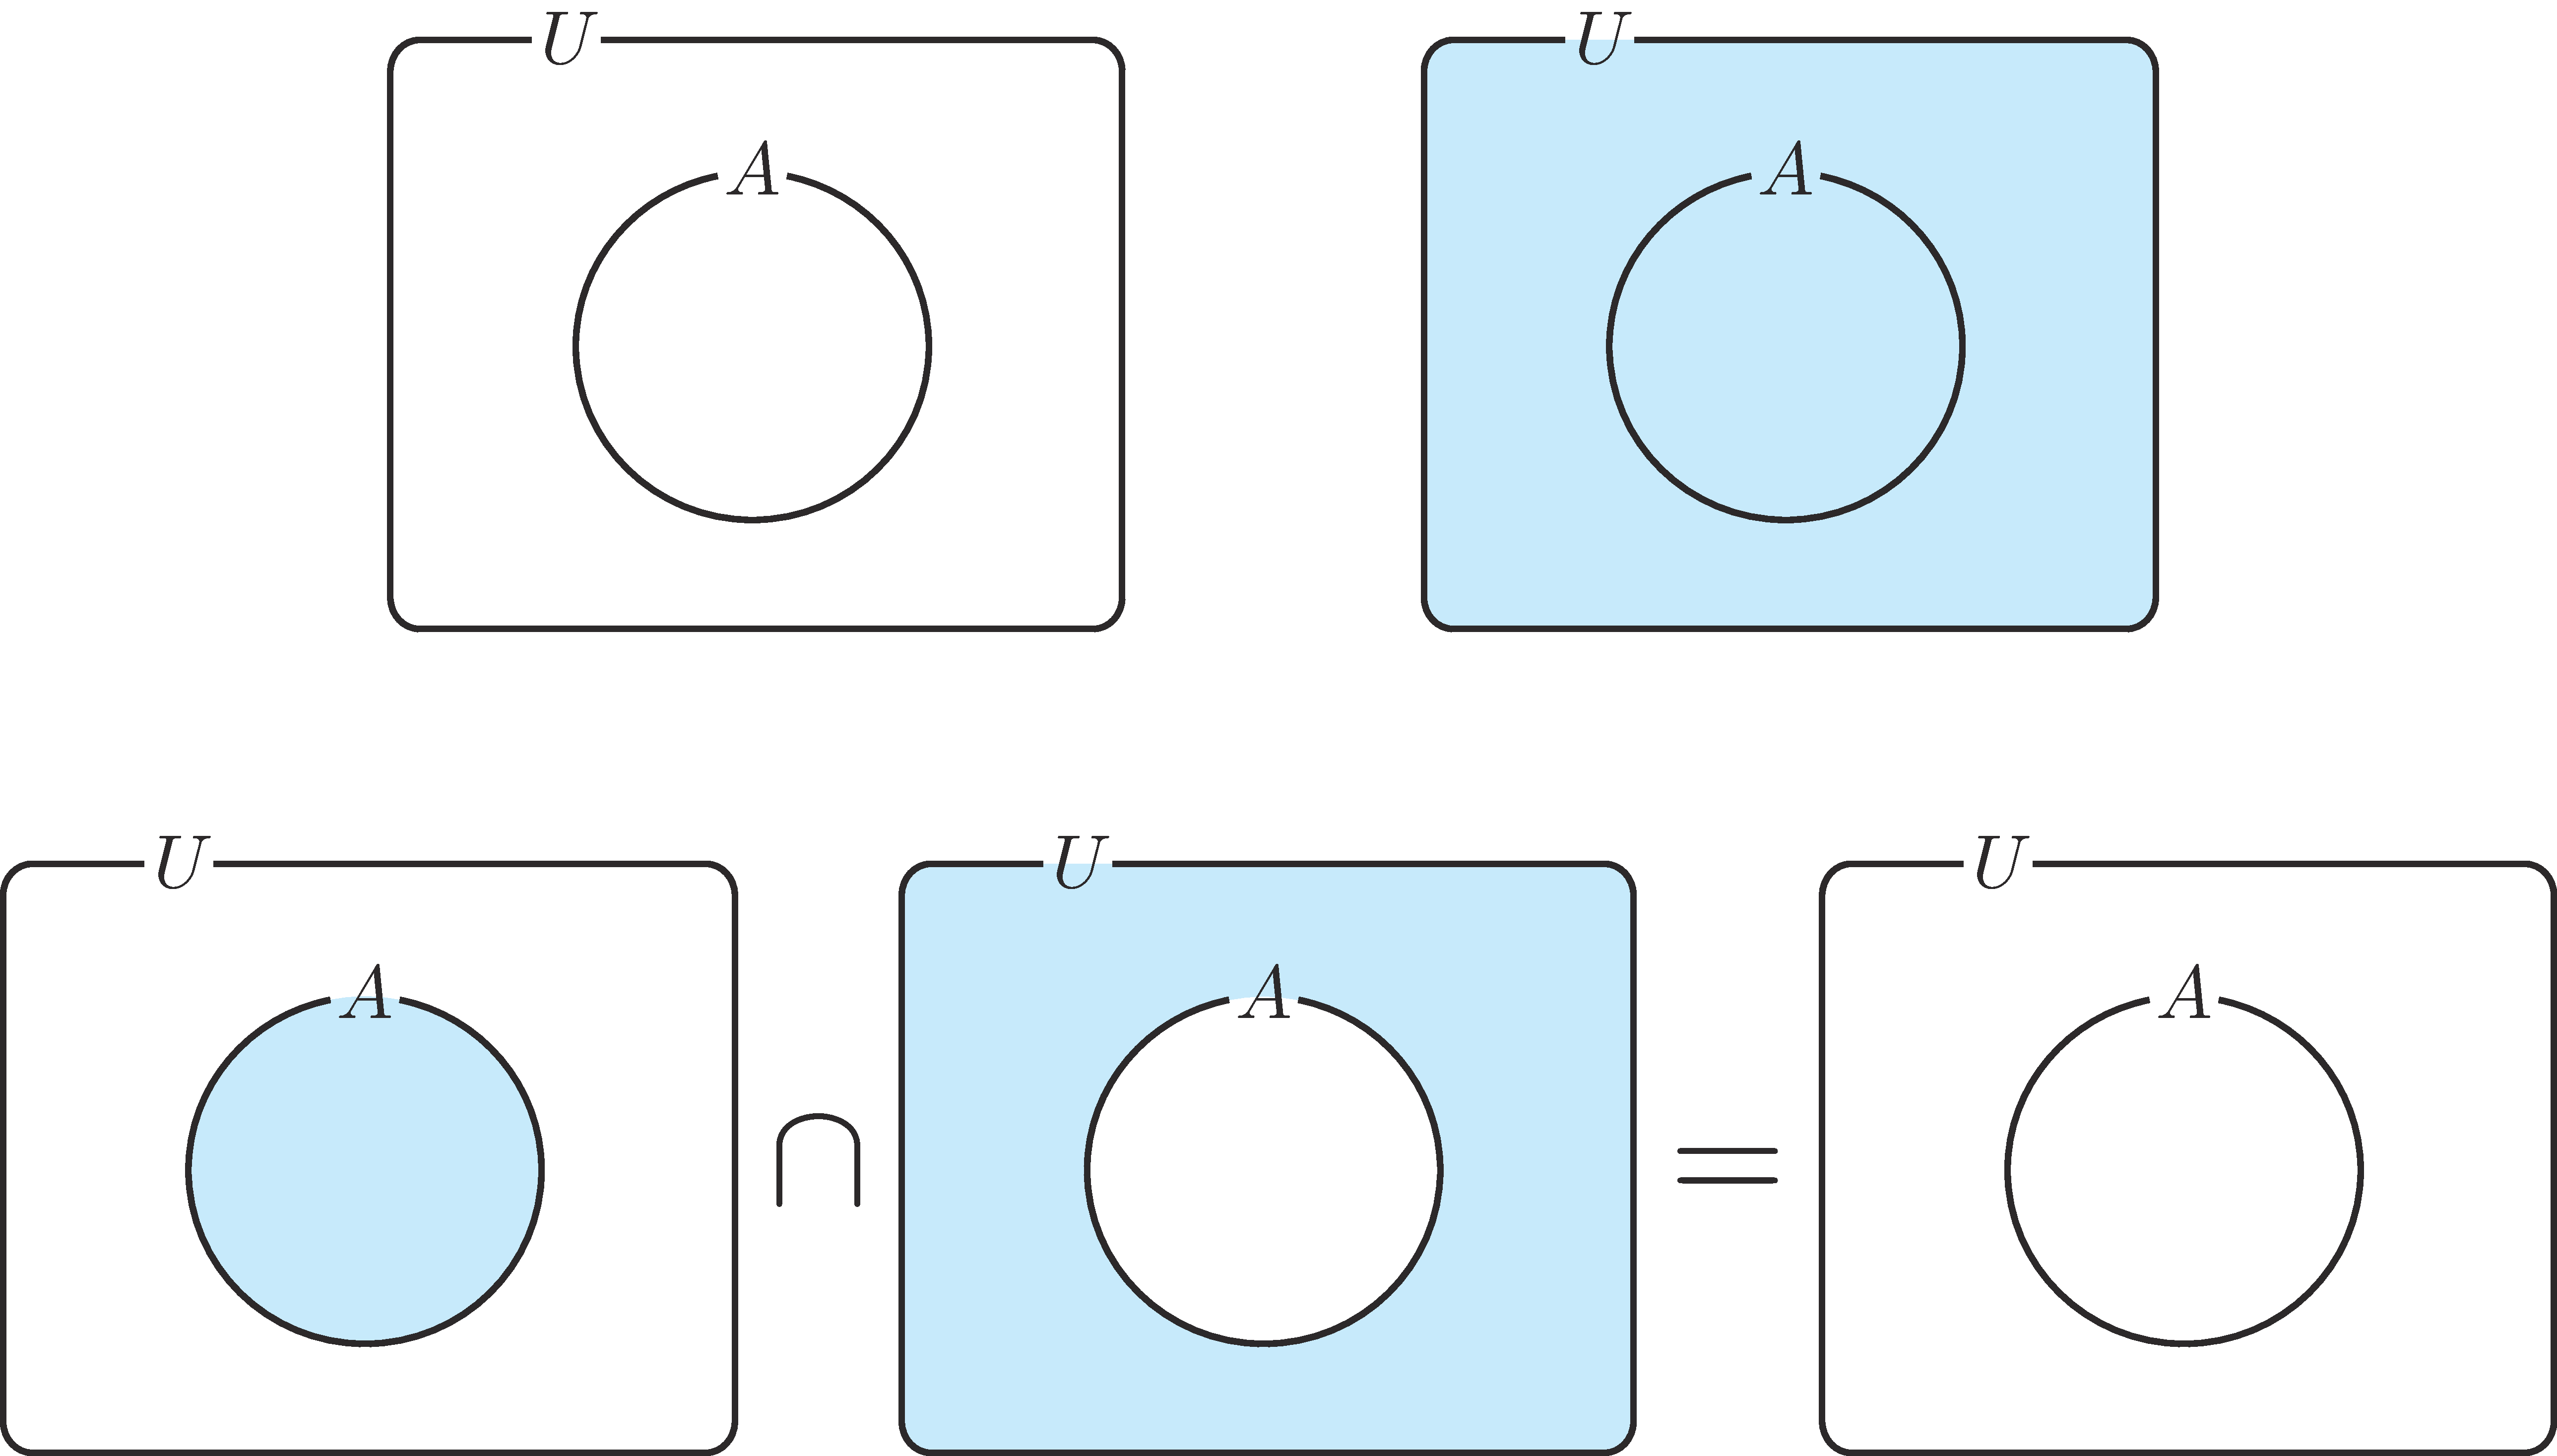
\includegraphics[scale=\pgfkeysvalueof{picsize}]{DBs/pic/zero_10_1.pdf}\
	\end{center}앞서 배운 연산을 이용하여 $U^C=\emptyset$, $\emptyset^C=U$,  $A \cap A^C = \emptyset$이 성립함을 보일 수 있습니다. 위 그림은 각각의 상황을 나타낸 것입니다.

\clearpage
\subsection{교환법칙}
일반적으로 두 집합 $A$, $B$에 대하여 다음이 성립하며, 이를 각각 합집합에 대한 \term{교환법칙}{}, 교집합에 대한 \term{교환법칙}{}이라고 합니다.
\begin{align*}
    A\cup B =& B \cup A\\
    A\cap B =& B \cap A
\end{align*}
\subsection{결합법칙}
일반적으로 세 집합 $A$, $B$, $C$에 대하여 다음이 성립하며, 이를 각각 합집합에 대한 \term{결합법칙}{}, 교집합에 대한 \term{결합법칙}{}이라고 합니다.
\begin{align*}
    \left( A\cup B \right) \cup C &= A\cup \left( B\cup C  \right) = A\cup B \cup C \\
    \left( A\cap B \right) \cap C &= A\cap \left( B\cap C  \right) =  A\cap B \cap C
\end{align*}

\subsection{분배법칙}
일반적으로 세 집합 $A$, $B$, $C$에 대하여 다음이 성립하며, 이를 집합의 연산에 대한 \term{분배법칙}{}이라고 합니다.
\begin{align*}
    A \cap\left( B \cup C  \right) &= \left( A \cap B \right) \cup \left( A\cap C \right)   \\
    A \cup\left( B \cap C  \right) &= \left( A \cup B \right) \cap \left( A\cup C \right) 
\end{align*}

\subsection{드모르간의 법칙}
일반적으로 전체집합 $U$의 두 부분집합 $A$, $B$에 대하여 다음과 같은 연산법칙이 성립합니다. 이를 \term{드모르간의 법칙}{}이라고 합니다.\mn{윗첨자 자리의 ${}^C$를 $A$, $B$에 각각 분배하고, 연산기호는 뒤집어준다고 생각하면 외우기 쉽습니다.}{}
\begin{align*}
\left( A \cup B \right)^C &=A^C \cap B^C \\
\left( A \cap B \right)^C &=A^C \cup B^C \\
\end{align*}


\mychapter{실수 체계와 구간표기법}{}

\section{실수 체계}
\subsection{자연수 집합 $\mathbb{N}$과 정수 집합 $\mathbb{Z}$}
\term{자연수}{}는 $1$, $2$, $3$, $4$, $\cdots$와 같은 수를 말합니다. \term{정수}{}는 $\cdots$, $-3$, $-2$, $-1$, $0$, $1$, $2$, $3$, $\cdots$과 같은 수를 말합니다.  자연수 전체를 원소로 갖는 집합을 $\mathbb{N}$, 정수 전체를 원소로 갖는 집합을 $\mathbb{Z}$라 부르기로 합시다.

\subsection{유리수 집합 $\mathbb{Q}$}
$n \in \mathbb{Z}$, $m \in \mathbb{Z}$이고 $n \ne 0$일 때, \term{유리수}{}는 $\dfrac{m}{n}$의 꼴, 즉 두 정수의 분수꼴로 나타낼 수 있는 수를 말합니다. 유리수 전체를 원소로 갖는 집합을 $\mathbb{Q}$라 부르기로 합시다. 이를 조건제시법으로 나타내면 다음과 같습니다.
\begin{align*}\mathbb{Q} = \conset[\bigg]{\dfrac{m}{n}}{$n\in\left(  \mathbb{Z}-\left\{ 0 \right\} \right)   $이고 $m\in \mathbb{Z}$}\end{align*}

유리수는 정수와 \term{정수가 아닌 유리수}{}로 나뉩니다. 정수가 아닌 유리수는 \term{기약분수}{}\mn{분수 $\dfrac{q}{p}$에서 $p$와 $q$의 최대공약수가 $1$인 경우,\mnpar 즉 $p$와 $q$가 서로소인 경우입니다.}{}로 나타내는 경우가 많습니다.
\begin{center} 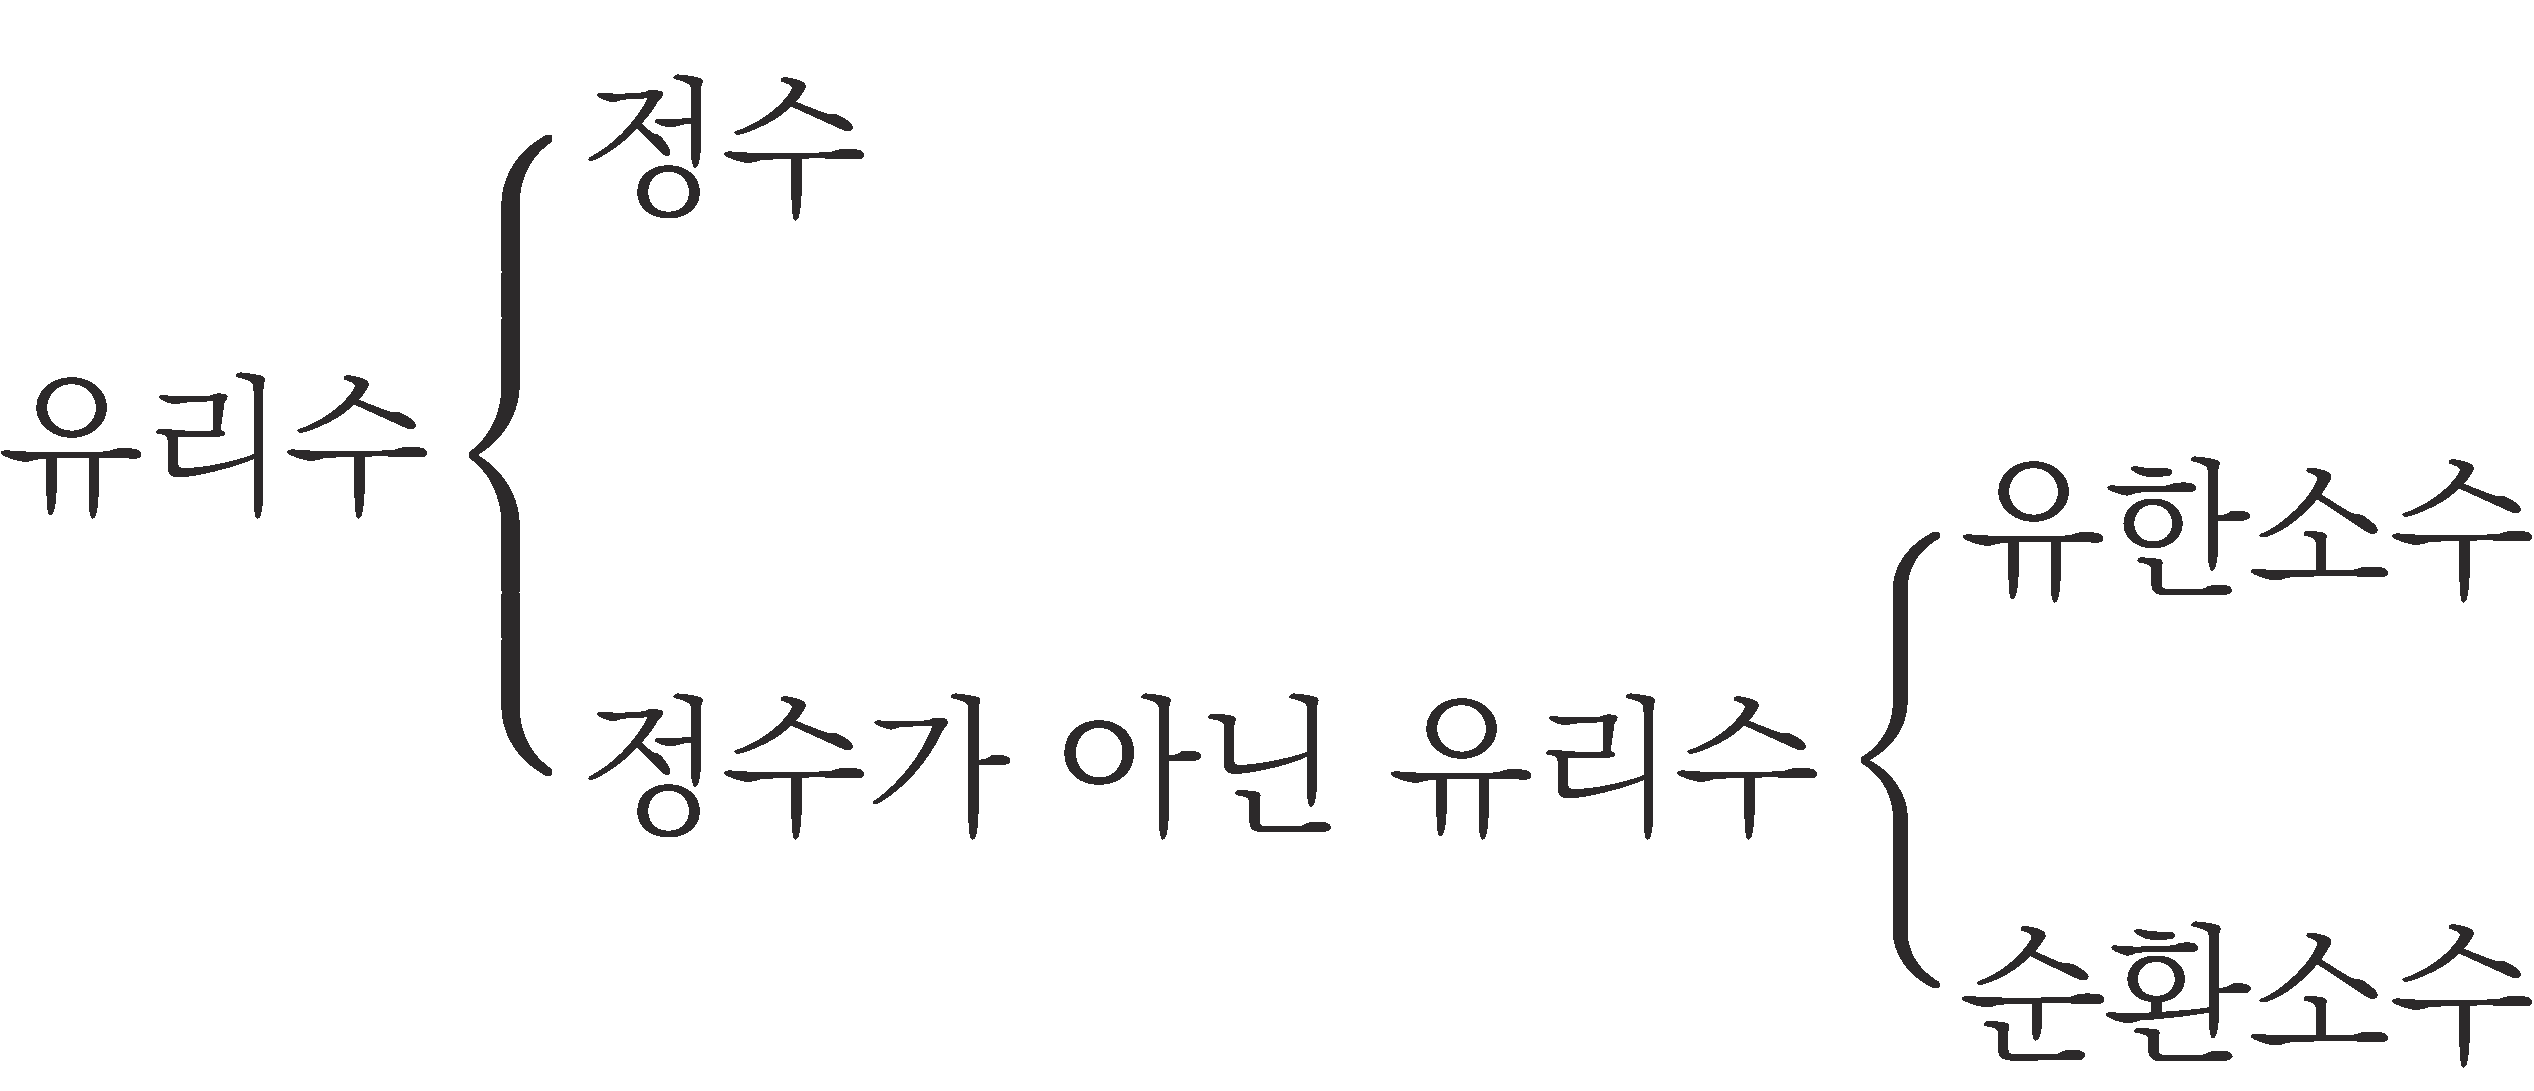
\includegraphics[scale=\pgfkeysvalueof{picsize}]{DBs/pic/zero_11.pdf}\
	\end{center}정수가 아닌 유리수는 \term{유한소수}{}와 \term{순환소수}{}로 나뉩니다. 유한소수는 $\dfrac{548}{1000}=0.548$과 같이 소수점 이후의 자리가 유한한 소수이고, 순환소수는 $\dfrac{1}{3}=0.33333\cdots=0.\dot3$, $\dfrac{919}{999}=0.919919919919\cdots=0.\dot91\dot9$, $\dfrac{53}{90}=0.5888\cdots=0.5\dot8$과 같이 소수점 이후의 일부 또는 전부의 자릿값이 규칙적으로 순환하는 무한소수입니다.\mn{규칙적으로 순환하지 않는 무한소수는 비순환소수라 하며, 이는 무리수입니다.}{}

\subsection{무리수 집합 $\mathbb{I}$}
$\pi = 3.141592\cdots$, $e = 2.7182818\cdots$와 같이 규칙적으로 순환하지 않는 무한소수를 \term{비순환소수}{}라 합니다. 모든 비순환소수는 \term{무리수}{}이고, 모든 무리수는 비순환소수입니다. 무리수의 집합을 $\mathbb{I}$라 부르기로 합시다.\mn{대학에서는 새로운 차집합 기호인 $\setminus$를 이용해 $\mathbb R \setminus \mathbb Q$라 표현하는 방법이 더 널리 쓰입니다.}{}

\subsection{실수 집합 $\mathbb{R}$}
유리수와 무리수를 통틀어 \term{실수}{}라고 합니다. 실수 전체를 원소로 갖는 집합을 $\mathbb{R}$라 부르기로 합시다. 이를 조건제시법으로 나타내면 다음과 같습니다. \begin{align*}\mathbb{R} = \conset{x}{$x\in \mathbb{Q} $ 또는 $x\in \mathbb{I}$}\end{align*}
\cleartorecto
\subsubsection{수직선}\begin{center} 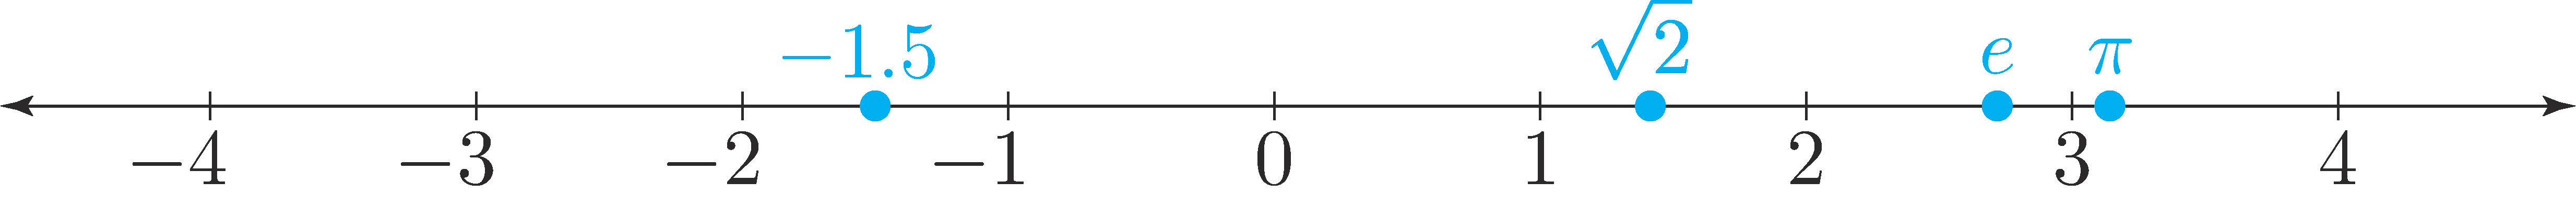
\includegraphics[scale=\pgfkeysvalueof{picsize}]{DBs/pic/zero_11_1.pdf}\
	\end{center}실수 집합은 직선, 실수 집합의 원소는 그 직선 위의 한 점에 대응됩니다. 이렇게 실수를 나타내는 직선을 \term{수직선}{}이라 합니다.
\section{실수를 바라보는 관점}

\subsection{정수의 여부 : 정수인가, 정수가 아닌가}
주어진 실수가 정수(자연수)일 때와 그렇지 않을 때는 다루는데 큰 차이가 두 가지 있습니다.

첫째, 정수(자연수)일 때에는 `주어진 수보다 큰 수 중에서 가장 작은 수'라는 개념과 `주어진 수보다 작은 수 중에서 가장 큰 수'라는 개념이 존재하지만, 실수에서는 존재하지 않습니다.

둘째, 범위가 한정되었을 때\mn{이를 테면 $-10<x<10$인 $x$} 정수(자연수)의 개수는 몇 개 되지 않으므로 따져야 할 경우가 한정되지만, 실수의 개수는 무수히 많으므로 경우별로 다룰 수는 없고 범위에 따라 다루어야 합니다.

\subsection{부호에 따라 : 양수인가, 음수인가, $0$인가}
수학에서는 주어진 실수의 부호가 무엇이냐가 중요한 경우가 굉장히 많습니다. 제곱할 때, 제곱근을 취할 때, 절댓값을 취할 때 부호에 주의해야 하는 것 또한 부호에 따라 그 값이 달라지기 때문입니다.
\clearpage

\section{구간표기법}
\subsection{구간표기법이 필요한 이유}
부등식의 해를 통해 어떤 실수인 변수가 취하는 범위를 나타낼 수 있습니다. 가령 $2$ 이상 $3$ 이하인 실수 $x$의 범위는 $2 \le x \le 3$입니다. 이 부등식의 해를 원소로 하는 집합 $X=\left\{x \mid 2 \le x \le 3\right\}$를 생각할 수도 있습니다.

그러나 매번 부등식이나 집합의 조건제시법으로 범위를 나타내기는 번거롭습니다. 부등식이나 집합 없이 간단하게 범위를 표현하기 위한 방법인 \iterm{구간표기법}{}을 배워봅시다. 

\subsection{범위의 양쪽 끝이 모두 제한되어 있을 때}
\begin{center} 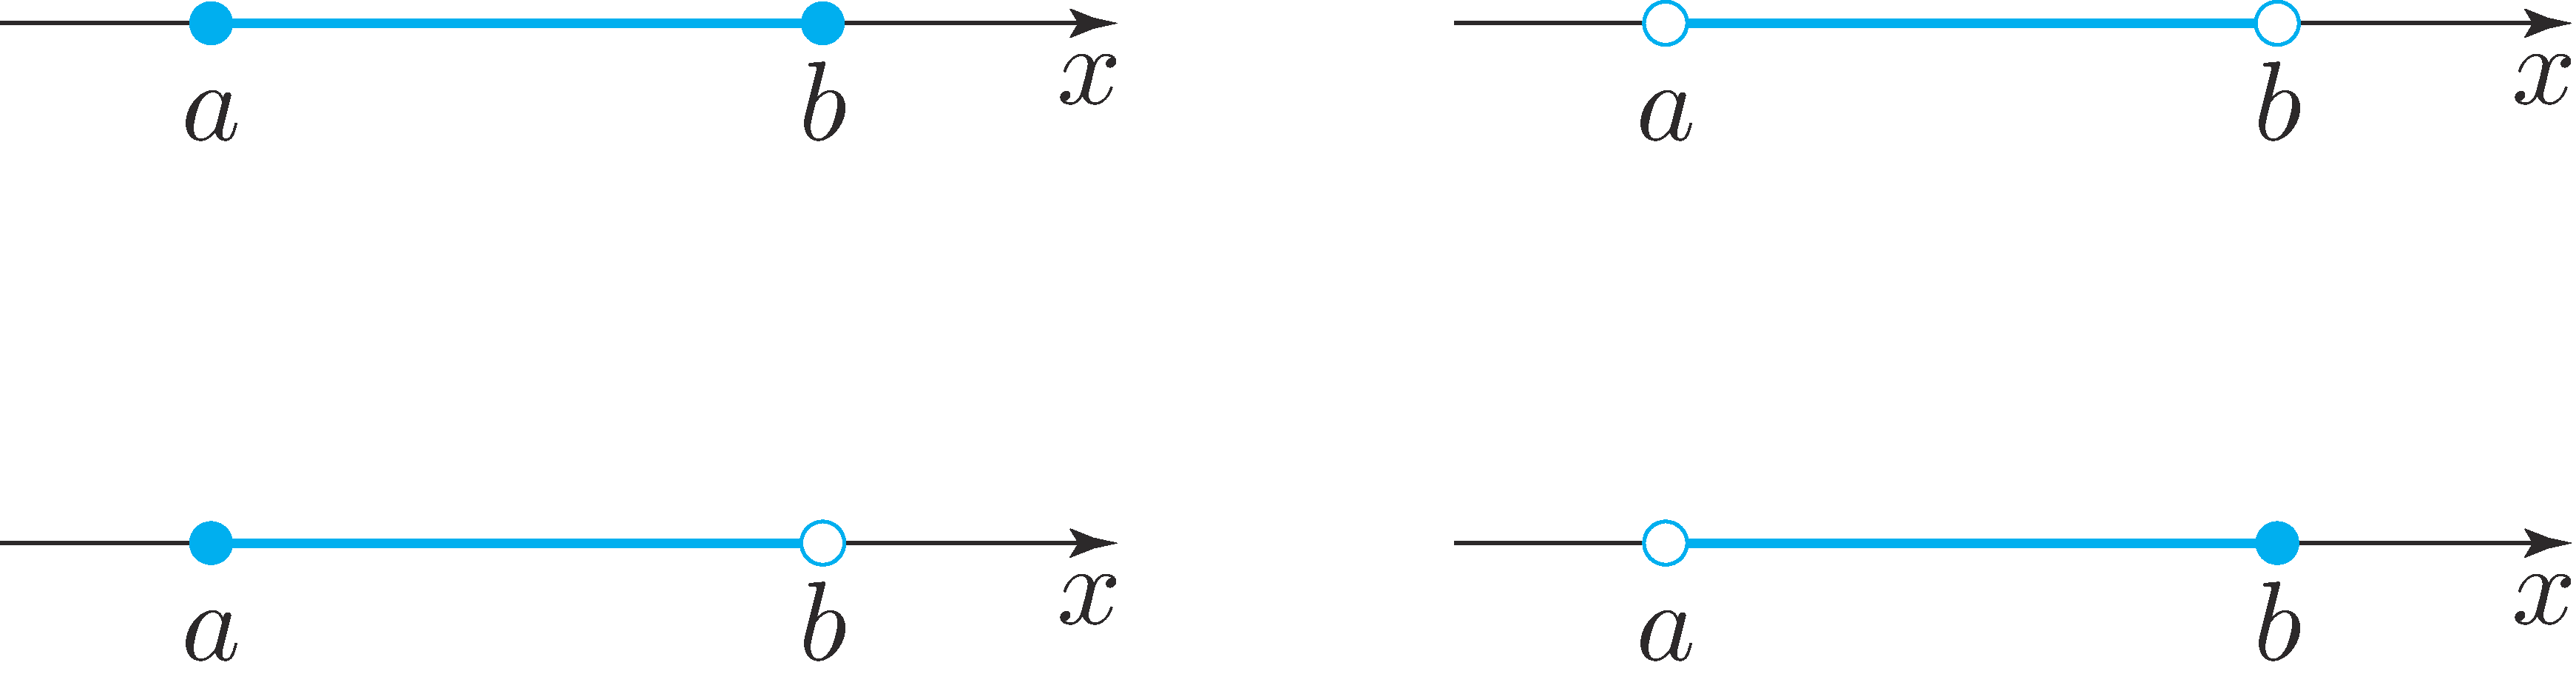
\includegraphics[scale=\pgfkeysvalueof{picsize}]{DBs/pic/zero_12.pdf}\
	\end{center}위 그림과 같이 범위의 양쪽 끝이 각각 서로 다른 실수 $a$, $b$ ($a<b$)로 제한되어 있을 때, $a$ 또는 $b$의 포함 여부에 따라 다음과 같이 $4$가지의 범위를 생각할 수 있습니다.
\begin{align*}
a \le x \le b, \: &&a < x < b, \\
a \le x < b, \: &&a < x \le b
\end{align*}
부등식 $a \le x \le b$를 만족하는 실수 $x$의 범위를 $\CCI{a}{b}$라 표기하고, 이를 `\term{닫힌구간}{} 에이 비'라 읽습니다. $a$를 \iterm{구간의 왼쪽 끝}{}, $b$를 \iterm{구간의 오른쪽 끝}이라고 부르기로 합시다.%\mn[-4em]{각각 하한(infimum, the greatest lower bound), 상한(supremum, the least upper bound)라는 해석학 용어가 있지만, 이를 이 책에서 사용하는 것은 부적절하다고 판단하여 주석을 통해 언급만 하고 넘어가겠습니다.}{}
부등식 $a < x < b$를 만족하는 실수 $x$의 범위를 $\OOI{a}{b}$라 표기하고, 이를 `\term{열린구간}{} 에이 비'라 읽습니다. 같은 방법으로 $a \le x < b$, $a < x \le b$를 각각 $\COI{a}{b}$과 $\OCI{a}{b}$라 정의할 수 있습니다. 이 둘을 일컬어 \term{반닫힌구간}{} 또는 \term{반열린구간}{}이라고 합니다.\mn{반닫힌(반열린) 구간은 잘 쓰이지 않다보니 둘을 명확히 구분하는 용어(이를테면 `여닫힌구간', `닫열린구간')가 정의되어 있지 않습니다.}{}

\subsection{범위의 한쪽 끝만 제한되어 있을 때 \& 무한대 $\infty$의 정의}
\begin{center} 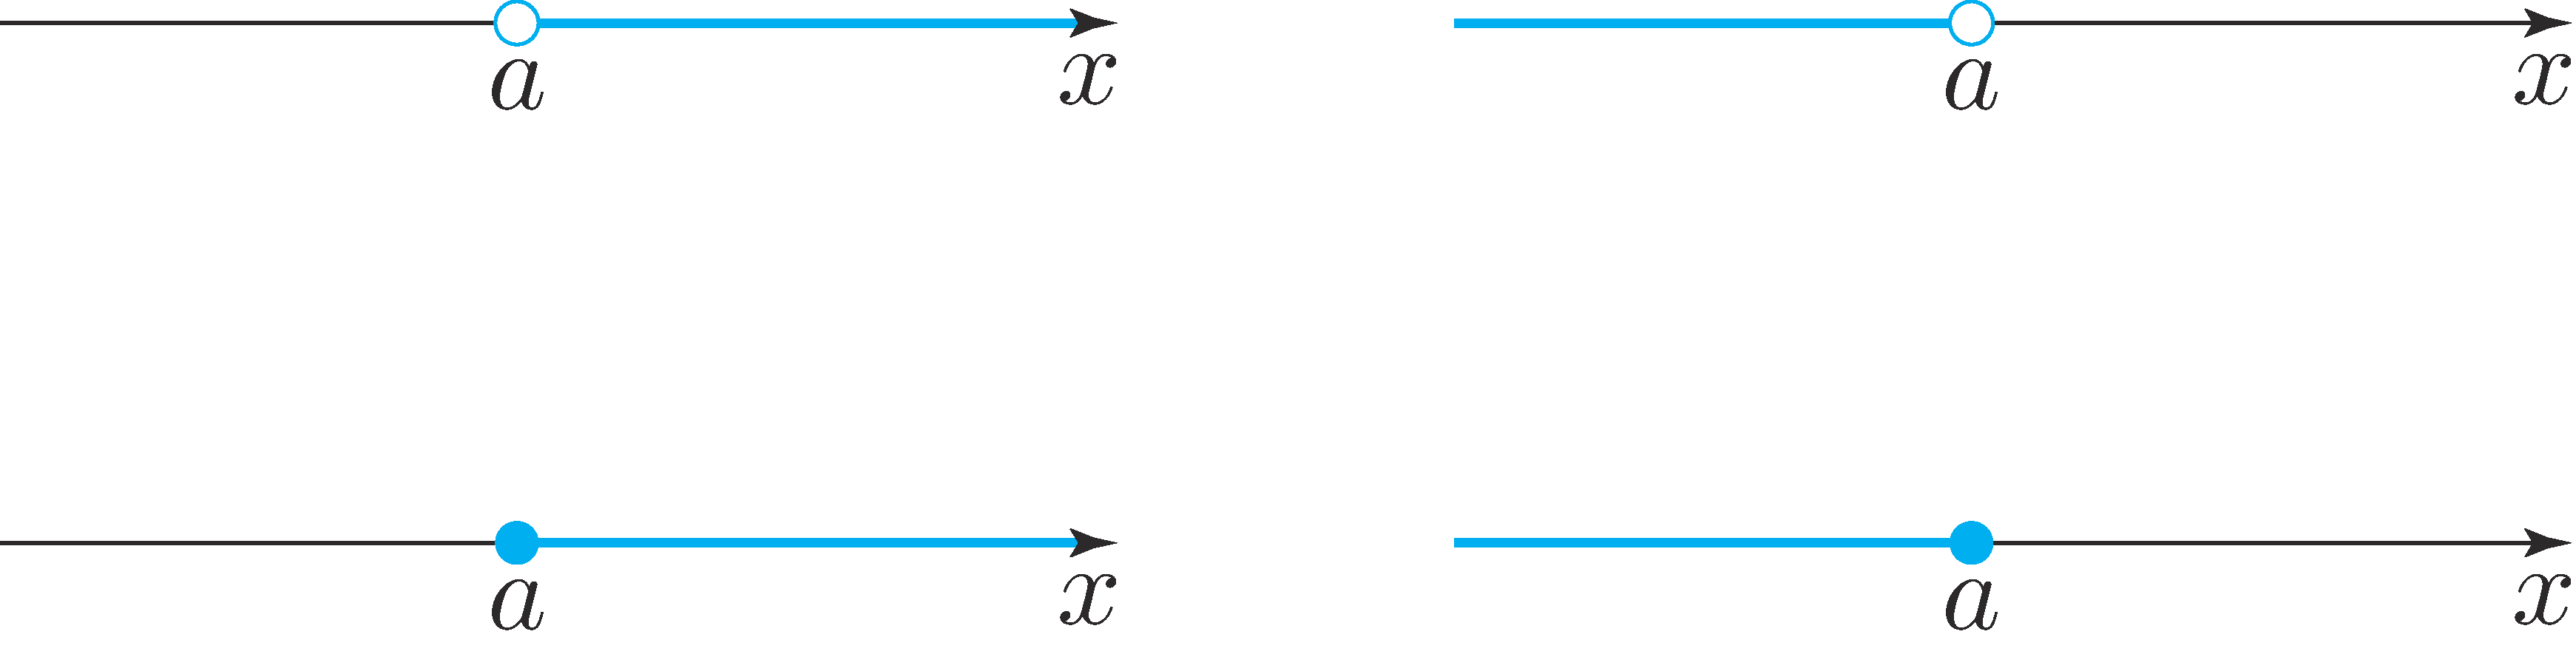
\includegraphics[scale=\pgfkeysvalueof{picsize}]{DBs/pic/zero_13.pdf}\
	\end{center}위 그림과 같이 범위의 한쪽 끝만 $a$로 제한되어 있을 때, $a$의 포함 여부에 따라 다음과 같이 $4$가지의 범위를 생각할 수 있습니다. %각각의 읽는 법은 따로 정해져 있지 않습니다.
\begin{align*}
    x  >  a, \: && x < a, \\
    x \ge a, \: && x \le a
\end{align*}\clearpage
$x>a$가 나타내는 구간의 왼쪽은 열려 있고, 구간의 왼쪽 끝은 $a$임이 확실합니다. 그러나 구간의 오른쪽 끝을 실수로 표기하기가 곤란합니다. 구간을 $\OCI{a}{b}$라고 표기하면, 이 표기는 부등식 $x>a$와 동일한 범위를 나타내지 않습니다. $c>b$인 실수 $c$가 존재하는데, $c$는 부등식 $x > a$의 해이지만, 구간 $\OCI{a}{b}$에는 포함되지 않기 때문입니다.\mn[-3\blskip]{이는 열린구간을 잡고 오른쪽 끝을 실수로 취했을 때에도 마찬가지입니다.}

이 실수 $c$를 포함하기 위하여 구간을 $\OCI{a}{c}$로 잡더라도 마찬가지입니다. $d>c$인 실수 $d$를 생각하면 모순이 발생하기 때문입니다. 이와 같이 부등식으로 나타낸 범위에 포함되는 모든 실수를 구간표기법으로 나타내려 하는 시도는 항상 실패할 수밖에 없습니다.\mn[-2\blskip]{잘 와닿지 않는다면 구체적인 숫자를 넣어 생각해보는 것이 좋습니다. 구간의 오른쪽 끝을 $1$억으로 잡으면 \mbox{$2$조를} 포함하지 못하고, \mbox{$2$조를} 포함하기 위해 구간의 오른쪽 끝을 $3$조로 잡으면 $10$조를 포함하지 못하는 것처럼, 어떤 실수를 잡더라도 더 큰 수가 존재하고, 그 수를 포함할 수 없습니다.}{}

따라서 $x>a$가 나타내는 범위를 표기하기 위하여 `그 어떤 실수보다도 큼'을 의미하는 기호인 $\infty$를 도입하고, $\OOI{a}{\infty}$라 표기합니다. 마찬가지로 $x \le a$가 나타내는 범위를 표기하기 위하여 `그 어떤 실수보다도 작음'을 의미하는 기호인  $-\infty$를 도입하고, $\OCI{-\infty}{a}$라 표기합니다. 그리고 $\infty$는 \term{무한대}{} 또는 \term{양의 무한대}{}, $-\infty$는 \term{음의 무한대}{}라 합니다.

주의할 점은, $\infty$와 $-\infty$는 절대로 실수가 아니라는 것입니다. 앞서 설명했듯 구간의 오른쪽 끝은 어떤 실수도 될 수 없으므로, $\infty$는 그 어떤 실수와도 같을 수 없습니다. 따라서 $\infty$는 실수가 아닙니다. $-\infty$ 또한 마찬가지입니다. 이를 달리 말하면, $\infty$와 $-\infty$는 $\mathbb{R}$의 원소가 아님에도 불구하고, $a \in \mathbb R$인 실수 $a$와 크기를 비교할 수 있는 특별한 개체\mn[2\blskip]{임의의 $a$에 대하여 $-\infty < a < \infty$입니다.}{}라 할 수 있습니다.

\subsection{실수 전체의 범위}
지금까지 설명한 내용을 바탕으로 생각하면, 실수 전체의 범위를 나타내기 위해서 구간의 왼쪽 끝과 구간의 오른쪽 끝을 각각 $-\infty$, $\infty$로 하여 $\OOI{-\infty}{\infty}$라 표기하는 것이 자연스럽습니다.
